%preamble
\documentclass[12pt,a4paper]{article}

% for subfigure 
\usepackage{caption}
\usepackage{subcaption}
% to have reference and index in table of content
\usepackage{tocbibind}
% to have index
\usepackage{makeidx}
\makeindex

\usepackage{graphicx}
%\graphicspath{{figures/}}
\usepackage{amsmath}

\usepackage{hyperref}

% for tabels
\usepackage{multirow}
\usepackage[table,xcdraw]{xcolor}
% for khafan enumrate
\usepackage[inline]{enumitem}
%%%%%%%%%%%%%%%%%%%%%%%%%%
% xepersian and fonts
\usepackage{xepersian}
\settextfont{XBZar}
\setdigitfont{XBZar}
%%%%%%%%%%%%%
\defpersianfont\titr[Scale=1]{XB Zar}
\defpersianfont\nastaliq[Scale=1.5]{IranNastaliq}
\defpersianfont\traffic[Scale=1]{XM Traffic}
%%%%%%%%%%%%%%%%%%%%%%%%%%

%body
\begin{document}
	% to make page number letter instead of number
	\pagenumbering{harfi}
	% to remove page number in this page
	\thispagestyle{empty}
	\vspace*{-45mm}
	\centerline{
\includegraphics[height=4cm]{figures/srulogofa.png}}
	\begin{center}
		
		\vspace{-3mm}
		دانشکده مهندسی کامپیوتر
		\\[.2cm]
		
		گروه هوش مصنوعی و رباتیکز
		\\[1cm]
		{\Large 
			\textbf{سمینار کارشناسی ارشد با عنوان}
		}
		\\[.4cm]
		\baselineskip=2cm
		{\titr
			\begin{huge}
				بررسی معیارهای فیزیولوژیکی چشمی و مغزی در سنجش بار شناختی در فرآیند یادگیری چندرسانه‌ای از طریق فیلم آموزشی
			\end{huge}
		}
		\\[1cm]
		{\Large
			{\traffic 
				استاد راهنما
			}
			\\[.7cm]
			{\Large \nastaliq دکتر رضا ابراهیم‌پور }
			\\[.7cm]
			{\Large\traffic  پژوهشگر
			}
		}
		\\[.6cm]
		{\Large \nastaliq امیرحسین اسعدی}
		\\[.2cm]
		بهار ۱۳۹۹
	\end{center}
% to go to new page
\newpage
% to change distance between lines
\baselineskip=1cm
% to create table
\tableofcontents

\newpage
\listoftables

\newpage
\listoffigures

\newpage
\baselineskip=.75cm
% to change pagenumbers in persian digit
\pagenumbering{arabic}

\section*{چکیده}
در عصر دیجیتال با پیشرفت فناری، روش‌های آموزش و یادگیری نیز دچار تغییر شده‌اند، استفاده از ارائه‌های چندرسانه‌ای یکی از این تحولات است. ساختن این آموزش‌‌های چند رسانه‌ای اگر بدون اصول باشد نه‌تنها کمکی به یادگیرنده نمی‌کند بلکه می‌تواند فشار ذهنی بیشتری برای وی ایجاد کند.
\\
بار شناختی باری است که بر روی حافظه‌ی فعال و در طول یک فرآیند شناختی توسط محرک شناختی ایجاد
می‌شود. هرچقدر که بار شناختی کمتر و در مقابل عملکرد دانش‌آموز پس از یادگیری بالاتر باشد، نشان‌دهنده‌ی فرآیند یادگیری مناسب است.
\\
از این رو اگر بتوان بار شناختی و عملکرد را در
حین آموزش و یا آزمون اندازه‌گیری کرد می‌توان میزان کیفیت ارائه‌های چندرسانه‌ای را به‌صورت غیرمستقیم سنجید. به عنوان مثال دو فرد را در نظر بگیرید که در یک آزمون عملکرد مشابه‌ای داشته باشند، در این حالت یادگیری‌ای مؤثر بوده که بار شناختی کمتری ایجاد کرده باشد.
\\
روش‌ها و دسته‌بندی های گوناگونی برای سنجش بار شناختی وجود دارد در این مطالعه به طور خاص سنجش بار شناختی با داده هایی که از چشم و مغز گرفته می‌شوند مورد بررسی قرار گرفته و سایر روش‌ها به صورت کلی‌تر بحث شده است.
% 1- introduction
\section{مقدمه}
\label{s:introduction}
امروزه با توسعه فناوری اطلاعات و ابزارهای نوین یادگیری و کاهش سهم آموزش رسمی در میان دانش‌آموزان و دانشجویان اهمیت نقش یادگیرنده و ابزارهای یادگیری مشخص می‌شود.
یکی از ابزار‌های نوین چندرسانه‌ای و فیلم‌های آموزشی است.کاهش فشار ذهنی یادگیرنده جزء اولویت‌های اصلی طراح چندرسانه‌ای آموزشی است.
فشار ذهنی می‌تواند از خود موضوع، رسانه انتقال و یا حاصل پردازش های شناختی یادگیرنده باشد.
\\
سنجش میزان بارشناختی ایجاد شده در یادگیرنده این امکان را می‌دهد تا بتوانیم با چیدمان و طراحی مناسب چندرسانه‌ای، کاهش بارشناختی یادگیرنده را مدیریت کنیم.
با ابزارهای مختلفی میتوان بارشناختی را سنجید که هریک مزایا و معایب خاص خود را دارد. در این پژوهش سعی شده است به طور خاص سنجش بار شناختی به وسیله داده‌هایی مختلفی که از چشم کاربر گرفته می‌شود مورد بررسی و مرور قرار گیرد.
\\
ساختار گزارش پیش‌رو با این شرح است در بخش
\ref{s:multimedia}
به اصول طراحی چندرسانه‌ای پرداخته می‌شود، این اصول با آزمایش های تجربی نشان داده شده‌ است که سبب کاهش میزان بارشناختی می‌شود. در بخش 
\ref{s:CognitiveLoad}
مفهوم بارشناختی و حافظه فعال ارائه می‌شود و سپس روش های متداول اندازه‌گیری بارشناختی معرفی خواهد شد.
در بخش 
\ref{s:eye}
به طور ویژه به سنجش بارشناختی به‌وسیله داده‌های چشمی و مغزی پرداخته می‌شود.
و در بخش 
\ref{s:data}
به نحوه پردازش داده‌ها و همچنین موارد مطالعه هریک پژوهش های مرتبط با داده‌های چشمی و مغزی در سنجش بار شناختی بررسی خواهد شد.
در نهایت در بخش
\ref{s:conclusion}
به نتیجه‌گیری و جمع‌بندی آن‌چه در این پژوهش مورد مطالعه قرار گرفته خواهیم پرداخت.
	
% 2- Principle of Multimedia Design
\section{گزارش پیشرفت دوره سه‌ماهه}
\subsection{فهرست فعالیت‌های انجام شده در این دوره (سه ماهه اول)}
\begin{enumerate}
	\item مطالعه‌ و پیاده‌سازی روش‌های پیش پردازش و استخراج ویژگی از سیگنال‌های مغزی
	\item مطالعه روش‌های تحلیل محتوای معنایی و زبانی
	\item  مطالعه روش‌های بررسی ارتباط میان سیگنال‌های مغزی و محتوای معنایی یک چندرسانه‌ای آموزش زبان  
\end{enumerate}
\subsection{شرح فعالیت‌ها و دستاورد‌های هر فعالیت در این دوره}
در این بخش شرح فعالیت‌ها و پیشرفت‌های انجام شده از آغاز پروژه تا تنظیم گزارش جاری بیان می‌شود. 
\begin{enumerate}
	\item
	{
		\begin{description}
			\item[عنوان فعالیت] مطالعه‌ و پیاده‌سازی روش‌های پیش پردازش و استخراج ویژگی از سیگنال‌های مغزی
			\item[دستاورد حاصل] داده‌های اخذ شده
			\cite{latifzadeh2020evaluating}
			با روش‌های جدیدتری از نویز‌های رایج سیگنال مغزی پاک سازی شدند. و ویژگی‌های متفاوتی نیز از آن‌ها استخراج شد.
			\item[ریز فعالیت‌ها]
			{
				\begin{enumerate*}
					\item یادگیری کار با نرم‌افزار EEGLAB که به منظور کار با سیگنال‌های مغزی طراحی شده است.
					\item یادگیری با افزونه‌های EEGLAB برای حذف نویز‌های متداول چون برق شهری، حرکت عضلات و پلک زدن طراحی شده‌اند.
					\item مطالعه روش‌های رایج و جدید برای استخراج ویژگی از سیگنال‌های مغزی.	
				\end{enumerate*}
			}
			\item[درصد پیشرفت (از ۱۰۰٪)] ۱۰۰	
			\item[توضحیات تکمیلی] در ادامه این گزارش آمده است.
	\end{description}
	}
	\item
	{
		\begin{description}
			\item[عنوان فعالیت] مطالعه روش‌های تحلیل محتوای معنایی و زبانی
			\item[دستاورد حاصل] دو روش متفاوت برای ارزیابی محتوای معنایی و زبانی چندرسانه‌ای بررسی، پیاده سازی و درنهایت ارزیابی شد.	
			\item[ریز فعالیت‌ها]
			{
				\begin{enumerate*}
					\item بررسی میزان پیچیدگی یک متن به لحاظ معنایی 
					\item میزان پیچیدگی یک متن به لحاظ ساختاری
					\item میزان فراوانی یک لغت در طول زمان
					\item ارزیابی روش‌های بیان شده
				\end{enumerate*}
			}
			\item[درصد پیشرفت (از ۱۰۰٪)] ۷۵ درصد	
			\item[توضحیات تکمیلی] در ادامه این گزارش آمده است.
		\end{description}
	}
	\item
	{
		\begin{description}
			\item[عنوان فعالیت] مطالعه روش‌های بررسی ارتباط میان سیگنال‌های مغزی و محتوای معنایی یک چندرسانه‌ای آموزش زبان\\
			
			\item[دستاورد حاصل] مشخص شدن مکان‌ها و زمانن‌هایی از مغز که بیشترین وابستگی را به معیار‌های زبانی دارند	
			\item[ریز فعالیت‌ها]
			{
				\begin{enumerate*}
					\item بررسی معیار‌های وابستگی میان دو سیگنال
					\item مطالعه پژوهش‌های مربوطه در این زمینه	
				\end{enumerate*}
			}
			\item[درصد پیشرفت (از ۱۰۰٪)] ۵۰ درصد	
			\item[توضحیات تکمیلی] در ادامه این گزارش آمده است.
		\end{description}
	}

\end{enumerate}
\subsection{گزارش تکمیلی فعالیت‌ها}
\subsubsection{پردازش سیگنال‌های مغزی}
در این قسمت سیگنال های خام اخذ شده 
\cite{latifzadeh2020evaluating}
با نرم افزار EEGLAB
\cite{delorme2004eeglab}
که یکی از بسته‌های متن باز متلب است پیش پردازش شدند. در ابتدا فرکانس‌های ۴۰ تا ۵۰ هرتز که مربوط به نویز برق شهری هستند حذف شدند. بعد از آن به کمک افزونه ASR برخی از اعمال چون: حذف بازه‌ای از سیگنال که در آن به مدت ۵ ثانیه ثابت باشد، فرکانس‌های زیر یک هرتز،‌ حذف کانال‌هایی که با کانال‌های اطراف خود همبستگی کمی دارند و بازه‌هایی از سیگنال که در آن پرش شدیدی وجود دارد.
\newline
 سپس به کمک افزونه‌ای که مولفه‌های سیگنال مغزی را استخراج می‌کند مولفه‌های غیر مغزی حذف شدند. این مولفه‌ها شامل پلک زدن، حرکت چشم‌ها، فرو بردن آب دهان، حرکت سر، نفس کشیدن و حرکت دندان‌ها هستند.
\subsubsection{تحلیل محتوای‌ معنایی و زبانی}
در این بخش متن گفتار چندرسانه‌ای آماده شده که زمان آن
$3'\text{:}41''$
و شامل ۷۸۲ کلمه بود با معیارهای متفاوتی مورد ارزیابی قرار گرفت. هدف از انجام این کار سنجش میزان پیچیدگی گفتار و فعالیت که ممکن است در مغز ایجاد کند بود. این کار با دو دسته معبار متفاوت انجام شد. نخست معیار کوماتریس 
\cite{castro2020validating}
استفاده شد در این معیار متن از از دو جنبه سهولت خواندن و سادگی ساختار مورد بررسی قرار گرفت.
\newline
سهولت خواندن خود از پارامتر‌هایی چون طول جمله، تعداد کلمات و تعداد سیلابس ها تشکیل شده است. و خروجی آن عددی در بازه ۱ تا ۱۰۰ است که هرچه بزرگتر باشد متن ساده تر بوده و برعکس. سادگی ساختار نیز متن را به لحاظ تعداد ضمیرها فاصله تا اسم مورد نظر واین دست موارد بررسی می‌کند. و خروجی آن همانند سهولت خواندن است. 
\newline
معیار بعدی فراوانی لغت
\LTRfootnote{Word Frequency}
است
\cite{brodbeck2018neural}.
در این معیار یک مخزن عظیم لغات در نظر گرفته می‌شود سپس میزان رخداد هر کلمه مجزا در آن محاسبه شده و اعلام می‌شود. به عنوان نمونه می‌توان تمام زیرنویس فیلم‌های موجود را یک مخزن عظیم داده در نظر گرفت و یا متن روزنامه‌های آنلاین. 
یک مسئله در این روش پیدا کردن زمان شروع و پایان گفتار یک کلمه است. برای این منظور ابتدا از شبکه عصبی که به این منظور آموزش دیده به نام Gentle استفاده شد و سپس برای دقیق شدن خروجی آن زمان‌های شروع و اتمام تمامی کلمات به صورت دستی با نرم‌افزار Praat تمیز شد. مزیت این روش نسبت به روش قبلی داشتن دقت زمانی بالا است.
\subsubsection{ارتباط میان سیگنال‌های مغزی و محتوای معنایی}
در این بخش معیار های متفاوت همبستگی
\LTRfootnote{Correlation}
مطالعه و مورد بررسی قرار گرفت. این معیار همبستگی شباهت میان دو مجموعه داده را می‌سنجد و خروجی آن عددی بین صفر تا یک است. هر چه این عدد به سمت صفر نزدیک‌تر باشد دو مشاهده مورد نظر همبستگی کمتری دارند و هرچه به سمت یک و منفی یک باشد همبستگی بیشتری دارند.
\newline
نوع دیگر از آن هبستگی کانونی
\LTRfootnote{Canonical Correlation}
است، که در آن همبستگی خطی میان چند مشاهده و چند مشاهده دیگر اندازه گیری می‌شود. می‌توان گفت این روش از این جهت که تمامی مشاهدات در نظر گرفته می‌شود و از هر کدام ضریبی در نظر گرفته شده دقیق‌تر است.
حال می‌توان ضریب‌ها در توپوگرافی مغز رسم نمود و نواحی مرتبط با پردازش کلمات در مغز را شناسایی نمود و یا با جابه‌جا کردن سیگنال در زمان با واحدهای کوچک مثلا پنجاه میلی ثانیه بررسی نمود که مغز در چه زمانی پس از نشان دادن محرک به آن پاسخ می‌دهد.
شکل 
کارهای انجام شده را نشان می‌دهد.
\begin{figure}[h]
	\centering
	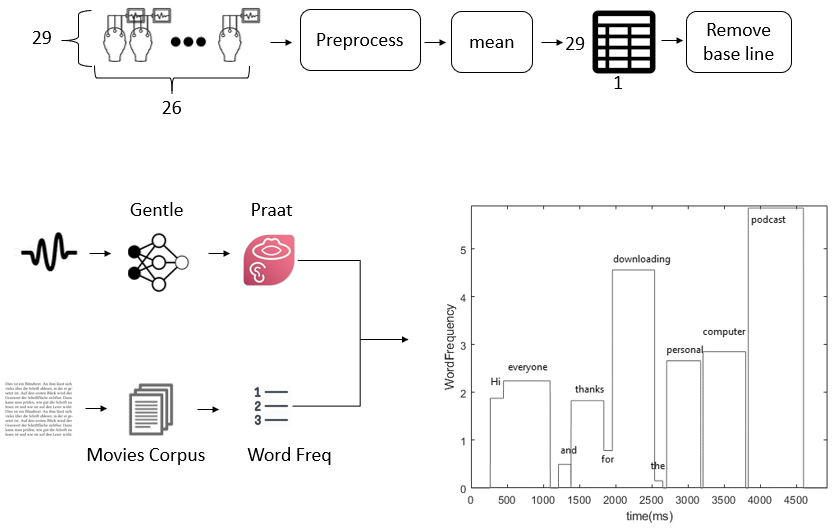
\includegraphics[width=0.8\linewidth]{figures/procedure}
	\caption[رویه‌ کار‌های انجام شده]{سیگنال‌های مغزی پس از پیش پردازش میانگین گرفته شده و ثانیه‌های ابتدایی آن که مربوط به حالت استراحت کاربر است حذف می‌شوند. از سوی دیگر گفتار و کلمات آن تحلیل می‌شوند و سیگنالی از فراوانی هر لغت در زمان آماده می‌شوند }
	\label{fig:procedure}
\end{figure}

\subsection{برنامه و زمان‌بندی ادامه اجرای پروژه}
انتظار می‌رود در سه ماهه دوم این اهداف و فعالیت‌ها محقق شوند:
\begin{enumerate}
	\item اتمام و جمع‌بندی رابطه میان گفتار چندرسانه‌ای به لحاظ زبانی و معنایی با فعالیت‌های مغزی
	\item بررسی جنبه‌های دیگر محتوای چندرسانه‌ای آموزشی همچون فیلم و فعالیت‌های مغزی
\end{enumerate}
% 3- Cognitive load and Measurements
\section{بار شناختی و معیارهای اندازه‌گیری}
\label{s:CognitiveLoad}
\subsection{مقدمه}
برای شناخت حافظه می‌توان از دو دید روانشناسی شناختی، و عصب شناسی می توان استفاده کرد. در دید عصب شناسی
\LTRfootnote{Neurology}
با اجزا و المان های واقعی مغز سروکار داریم ولی در دید روان شناسی شناختی با مدل سازی سر و کار داریم که در تلاش برای شناخت و ذهن است، پس باید به خاطر داشته باشیم در روانشناسی شناختی مدل ها مفید هستند نه درست.
اتکینسون
\cite{atkinson1968human}
مدل حافظه کوتاه مدت و حافظه بلند مدت و حافظه حسی را مطرح کرد. در مدل او حافظه از سه بخش اصلی تشکیل شده است. اطلاعاتی که توسط حواس ما (بویایی، بینایی، شنوایی، لامسه و چشایی)برای مدت بسیار کوتاهی، کمتر از یک ثانیه
\cite{sperling1960information}
 ثبت می‌شوند. بسیاری از آنها حذف و بخش که مورد توجه مغز گرار می‌گیرد به حافظه کوتاه مدت منتقل می‌شود، حافظه کوتاه مدت نیز نمی‌تواند برای طولانی مدت آنها را در خود نگه دار مگر مدام آن را تکرار کند.
 \\
 اینکه چه اطلاعاتی از حافظه حسی به کوتاه مدت منتقل می‌شوند بسته به آن است که به چه چیز متوجه هستیم و منتظر دریافت آنیم.
 ویژگی مهمی که برای حافظه کوتاه مدت در نظر گرفته می‌شود مفهوم رمزگذاری
 \LTRfootnote{Encoding}
است، رمز گذاری به شکل های مختلفی انجام می‌شود.
\begin{itemize}
	\item کد معنایی 
	\LTRfootnote{Semantic Code}
	هنگامی که یک مفهوم به خاطر سپرده می‌شود.
	\item کد صوتی
	\LTRfootnote{Phenological Code}
	هنگامی که یک مفهوم در قالب آوا و صوت به خاطر سپرده می‌شود.
	\item کد حرکتی
	\LTRfootnote{Motor Code}
	هنگامی که حرکات بدن به خاطر سپرده می‌شوند.
	\item کد تصویری
	\LTRfootnote{Visual Code}
	هنگامی که یک مفهوم در قالب تصویر به خاطر سپرده می‌شود.
\end{itemize}

\begin{figure}[htbp]
	\centering
	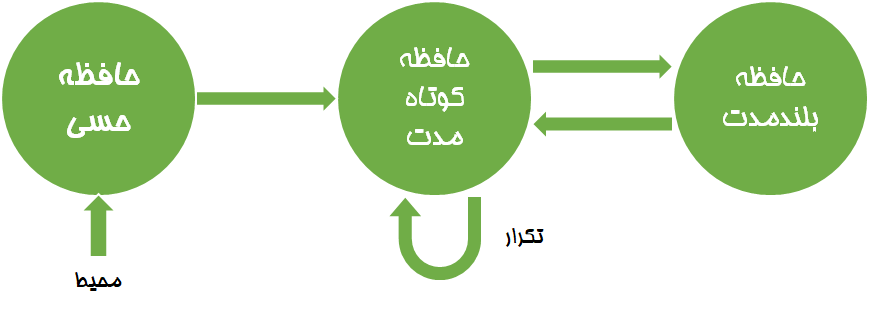
\includegraphics[width=0.7\linewidth]{figures/memory}
	\caption[تصویر مدل حافظه]{تصویر مدل ارائه شده توسط اتکینسون}
	\label{fig:memory}
\end{figure}

برای اندازه گیری ظرفیت حافظه از واحی به نام بسته اطلاعاتی
\LTRfootnote{Chunk}
استفاده می‌شود.
گفته می‌شود ظرفیت حافظه کوتاه مدت بین ۵ تا ۹ واحد اطلاعاتی است، این ظرفیت بین انسان ها متفاوت بوده جالب آنکه در یک فرد در ساعت‌های مختلف شبانه روز و حالات روحی مختلف متفاوت است.
\\
در دو دهه گذشته پیشنهاد شده است حافظه کوتاه مدت را نباید تنها محل ذخیره سازی و بازیابی اطلاعات در نظر گرفت. اگر فرض کنیم علاوه بر اینها در کوتاه مدت نیز می‌تواند با اطلاعات کار کند و آنها را پردازش کند، به مدل واقعی تر نزدیک شده‌ایم.از این رو مفهوم حافظه فعال
\LTRfootnote{Working Memory}
مطرح شده است.
\\
در این فصل، ابتدا نظریه‌ی بار شناختی معرفی و در ادامه روش‌های مختلف سنجش بارشناختی در چهار دهه گذشته بیان می‌شود.
\cite{sweller2011measuring}

\subsection{نظریه‌ی بار شناختی}
در روانشناسی شناختی، به میزان استفاده از منابع حافظه فعال گفته می‌شود. این نظریه بر مبنای ساختار شناختی انسان،‌دانش جدیدی درباره مشخصه های حافظه فعال، بلند مدت و رابطه بین این دو ارائه می‌کند.
\cite{sweller2019cognitive}
نظریه بارشناختی، سعی دارد چگونگی تاثیر بار ناشی از پردازش اطلاعات بر توانایی یادگیری اطلاعات جدید در حافظه فعال و بلند مدت را توصیف کند.
\\
پیش فرض اصلی این نظریه، محدود بودن حافظه فعال است که سبب محدودیت در توان پردازش شناختی انسان می‌شود. به طوری که تنها اطلاعات محدودی را می‌تواند در هر لحظه پردازش نماید. اگر تقاضای غیر ضروری به سیستم شناختی افزایش یابد سبب افزایش بار شناختی خواهد شد و اگر بار شناختی بیش از حد افزایش یابد سبب عدم انتقال مناسب اطلاعات و یادگیری مطلوب خواهد شد. چنین تفاضاهای غیر ضروری‌ای می‌تواند ناشی از روش‌های نامناسب آموزشی و یا پیچیدگی ذاتی محتوای تدریس شده باشد. از این رو جهت افزایش کیفیت یادگیری بهتر است بار شناختی را به نحوی مدیریت کرد که پردازش بی ارتباط با یادگیری کمینه و پردازش شناختی ذاتی یادگیری بهینه شود.
\cite{sweller2019cognitive}
\\
محدودیت حافظه کاری با توجه به اطلاعات جدید هنگام یادگیری یک تنگنا، به حساب می‌آید و تنها ۲
$\pm$
۷
عنصر اطلاعات می‌تواند در حافظه فعال نگهداری شود، این در حالی است که اگر اطلاعات نیاز به پردازش نیز داشته باشند کمتر نیز خواهد شد.
\\
به عنوان نمونه عناصر وابسته‌ای که باید باهم ترکیب شود را در یادگیری یک برنامه نوشته شده برای اجرای الگوریتم جستجوی دودویی در نظر بگیرید. یادگیری این برنامه به صورت ذاتی بسیار پیچیده تر از دستورات برنامه به صورت جداگانه است. زیرا برنامه به صورت ترکیبی از دستورات برنامه نویسی و چندین واحد اطلاعات است. در حال که دستورها را می‌توان به صورت ترتیبی از اطلاعات منفرد یاد گرفت. 
\\
بنابراین هرچه تعداد عناصر اطلاعات در تعامل با یکدیگر، در یک فعالیت بیشتر باشد، آن فعالیت سخت تر بوده و بار ذاتی بیشتری را به حافظه فعال وارد می‌کند. با این حال اطلاعاتی که پیش از این، در حافظه بلند مدت، به شکل الگوی‌های شناختی
\LTRfootnote{Cognitive schemas}
ذخیره شده است، می‌تواند بار شناختی را کاهش دهد. زیرا این الگو‌ها می‌توانند به صورت یک واحد اطلاعاتی در حافظه فعال استفاده شود، از این رو داشتین دانش پیشین در رابطه با یک فعالیت،‌ بار شناختی را کاهش می‌دهد. همچنین اگر یک فعالیت و جنبه های وابسته به آن به صورت تکراری تمرین شوند، الگو گیری شناختی خودکار شده و دیگر نیاز به پردازش کنترل شده ندارد به همین دلیل منابع بیشتری در حافظه فعال آزاد خواهند بود.
\cite{antonenko2010using}
در شکل 
\ref{fig:cognitionpatern}
الگوی شناختی دستگاه پردازش اطلاعات ذهن انسان 
در  هنگام  یادگيری  چندرسانهای  را  مشاهده می‌کنید. كلمه‌ها و  تصاویر  از  دنيای  خارج  به  صورت  ارائه 
چندرسانهای، از طریق گوش‌ها و چشم‌ها وارد حافظه حسی می‌شوند. تصاویر و متن‌های چاپی از طریق 
حافظه حسی دیداری و كلمات صحبت و دیگر صداها از طریق حافظه حسی شنيداری وارد حافظه‌ی كاری
می‌شوند. كار اصلی یادگيری چندرسانه‌ای در حافظه‌ی كاری انجام می‌شود. در این گام، الگوهای كلامی 
و تصویری (سمت راست) با استفاده از محتواهای خام وارد شده (سمت چپ) ساخته می‌شوند. دانش 
ساخته شده در حافظه‌ی كاری پس از ادغام با دانش پيشين در حافظه بلندمدت جای می‌گيرد.
\begin{figure}[htbp]
	\centering
	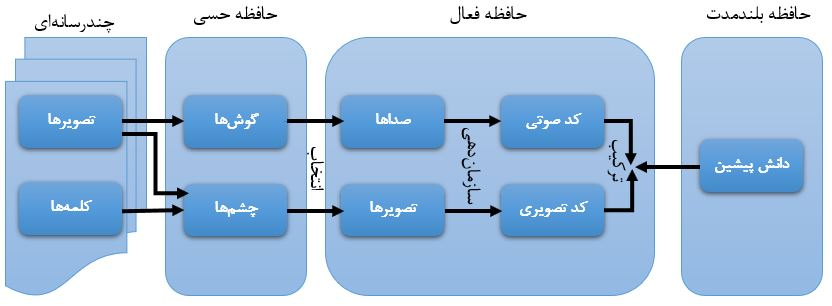
\includegraphics[width=\linewidth]{figures/cognition_patern}
	\caption[مدل الگوی شناختی یادگیری]{مدل الگوی شناختی یادگیری چند‌رسانه‌ای}
	\label{fig:cognitionpatern}
\end{figure}


\subsubsection{انواع بار شناختی}
بر اساس نظریه بارشناختی، در سه نوع بار شناختی را می‌توان مورد بررسی قرار داد: بار ذاتی
\LTRfootnote{intrinsic load}
، بار فرعی
\LTRfootnote{extraneous load}
و بار وابسته
\LTRfootnote{germane load}
.
\\
\textbf{بار ذاتی}
به پیچیدگی ذاتی محتوای در حال پردازش و نحوه تعامل عناصر اطلاعاتی گفته می‌شود که متناسب با سطح دانش پیشین یادگیرنده از موضوع اعمال می‌شود. به دلیل مشخصه های شناختی انسان، تعیین پیچیدگی اطلاعات پردازش شده دشوار است
\\
\textbf{بار فرعی}
بار ذهنی غیر ضروری است که توسط طراحی،‌ نا مناسب شناختی و ارائه‌ی نامناسب اطلاعات ایجاد می‌شود.
\\
\textbf{بار وابسته}
به عنوان منابع شناختی مورد نیاز برای دست‌کاری بار ذاتی تعریف می‌شود. این نوع بار هنگامی ایجاد می‌شود که ارائه اطلاعات برای یادگیری،‌ مفاهیم جدید و یا ماندگاری آن‌ها در ذهن طراحی شده‌باشد.
\cite{antonenko2010using}
\subsubsection{سطوح مختلف بارشناختی}
در تعریفی دیگر می‌توان گفت، بار شناختی را می‌توان اینگونه بیان نمود: باری که در طول یک فرآیند شناختی، بر حافظه فعال توسط محتوای آموزشی تحمیل می‌شود. این بار در سطوح مختلف شامل
\\
\textbf{بار لحظه‌ای}
\LTRfootnote{Instantaneous load}
نشان دهنده تغییرات بار شناختی از نخستین تا آخرین لحظه در طول یک یا چند فعالیت شناختی. این بار شناختی پایه‌ای ترین سطح سنجش بارشناختی است از این رو سایر سطح بارهای شناختی بر مبنای آن تعریف می‌شود.
\\
\textbf{بار بیشینه}
\LTRfootnote{Peak load}
،به بیشترین مقدار بار لحظه‌ای در هنگام اجرای یک فعالیت گفته می‌شود. بار بیشینه را می‌توان از طریق مقایسه بزرگی تمامی بارهای لحظه‌ای بدست آورد.
\\
\textbf{بار میانگین}
\LTRfootnote{Average load}
نمایانگر شدت بار متوسط در طول اجرای یک فعالیت و معادل مقدار میانگین بار لحظه‌ای، یا بار تجمعی در واحد زمان است.
\\
\textbf{بار تجمعی}
\LTRfootnote{Accumulated load}
مجموع مقدار باری که در طول اجرای یک فعالیت، یادگیرنده تجربه می‌کند.
\\
\textbf{بار سراسری}
\LTRfootnote{Overall load}
باری تجربی که بر پایه‌ی روند فعالیت، اعمال می‌شود. اعتقاد بر این است که بار سراسری نمایانگر دریافت شخص از تلاش ذهنی خود است.
\\
از آنجا که بار شناختی مستقیماً به مدت فعالیت بستگی دارد، هم بار میانگین و هم بار تجمعی برای تخمین اثرات طراحی آموزشی استفاده می‌شود.
\cite{antonenko2010using}
در شکل 
می‌توانید هریک از سطوح بارشناختی را مشاهده نمایید.
\begin{figure}[htbp]
	\centering
	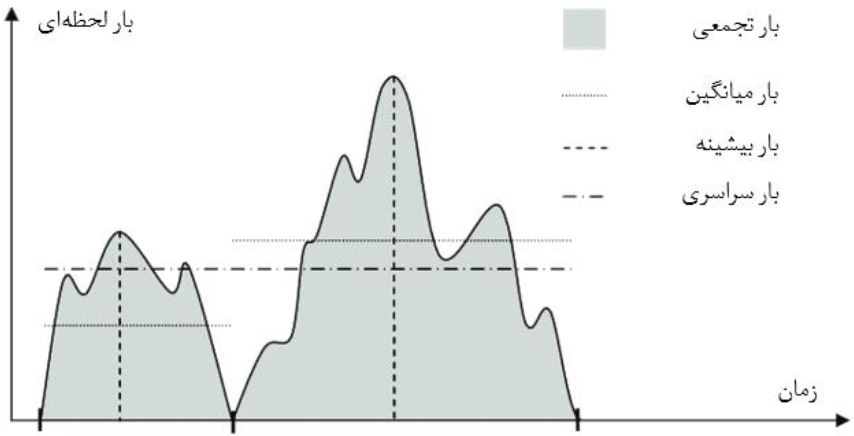
\includegraphics[width=0.7\linewidth]{figures/cl_levels}
	\caption[سطوح مختلف بار شناختی]{طرحی از سطوح مختلف بار شناختی شامل: تجمعی، میانگین، بیشینه و سراسری.}
	\label{fig:cllevels}
\end{figure}


\subsection{معیارهای سنجش بار شناختی}
هنگامی که از بار شناختی صحبت می‌کنیم یک سوال مهم راه‌های سنجش و اندازگیری آن است، این مقوله نقش جدی در پژوهش های مبتنی بر نظریه‌ي بار شناختی ایفا می‌کند از طرفی کاربردهای که در طراحی آموزش کارآمد دارد سبب اهمیت ویژه آن می‌شود.
\cite{korbach2017measurement}
\\
در ادامه روش های بیان شده در ادبیات اندازه گیری بار شناختی را مرور خواهیم کرد.

\subsubsection{کاربرد‌های سنجش بارشناختی}
علاقه به استفاده از فناوری شناختی در عمل بالینی در سالهای اخیر افزایش یافته است. کاربردهای متداول استفاده از آزمایشهای شناختی برای ارزیابی نقص در هنگام بروز اختلال‌هایی در سیستم عصبی مرکزی است. به طور نمونه چند نمنه عنوان مثال ذکر می‌کنیم:آسیب دیدگی سر، اسکیزوفرنی، سوء مصرف طولانی مدت الکل، بیماری آلزایمر و اختلال‌های مرتبط با آن، هستند.
\\
علاوه بر این ، از آنجا که مهارت های شناختی با زندگی روزمره و فعالیت های اجتماعی همراه است،ارزیابی شناختی می تواند در غربالگری  و پایش بیماران ترخیص‌شده و در ساخت راهکارهای توانبخشی فردی سودمند باشد.
\\
از آنجا که بار شناختی در نتیجه حافظه کاری محدود در حین کار ایجاد می شود ، اندازه گیری بار شناختی بر روی بیماران در آزمایش‌های شناختی می تواند بینش هایی را برای معالجه بیمار ارائه دهد.
به عنوان مثال، بار شناختی زیاد و مدت زمان محرک کوتاه برای ایجاد تمایز برای بیماران اسکیزوفرنی پیدا شد.
سایر کاربردها شامل کاهش خطاهای پزشکی به دلیل بار زیاد حافظه پزشکان در اورژانس است.
مطالعات نشان داده است که وقفه ها (باعث از بین رفتن اطلاعات) و چندکار را هم‌زمان انجام دادن باعث افزایش بار شناختی می شود که به خطاهای پزشکی کمک می کند.
راه حل های ارائه شده شامل استفاده از ابزارهای الکترونیکی برای پشتیبانی از روند به صورت تطبیقی در محل کار و ارائه آموزش های مؤثر جهت کاهش بار شناختی در محل کار است.
تمرکز دیگر بر ارزیابی سیستم های اطلاعات بالینی است. رویکردها مبتنی بر مهندسی کردن قابلیت‌ها و موارد استفاده و   تجزیه و تحلیل وظیفه شناختی است تا اطمینان حاصل شود که  در حالی که کاربران در حال انجام وظایف هستند کمترین بار شناختی در استفاده از چنین سیستم‌هایی مصرف شود.
\subsubsection{معیار های غیرمستقیم سنجش بارشناختی}
در نخستین روزهای ارائه نظریه بارشناختی، بار شناختی به صورت مستقیم اندازه گیری نمی‌شد یکی از اولین روش‌ها بر اساس نتایج آزمایش‌ها،‌ ارتباط میان بار شناختی و حل مسئله بود، از این رو چندین روش برای ارزیابی غیر مستقیم بار شناختی مورد استفاده قرار گرفت.
\cite{sweller2011measuring}
\paragraph{الگوهای محاسباتی}
نخستین پژوهش‌ها تمرکز خود را بر روی ناکارآمدی حل مسئله به عنوان راهبرد یادگیری تمرکز کرده‌ بودند. این گونه فرض می‌شد که کاوش بر روی مسئله سطح بالا منجر به بار بیشتر بر روی حافظه فعال و تلاش برای حل مسئله سطح پایین منجر به بار حافظه فعال کمتر خواهد شد.
\cite{sweller2011measuring}
\\
در یک مجموعه از آزمایشها ،سویلر و همکاران نشان دادند كه راهبرد یادگيری كه شامل جستجوی
قابل توجه در حل یک مسئله است، منجر به یادگيری پایينتری نسبت به مسئله‌ای كه نيازمند جستجوی
بالاتری داشت،  شده  است. سویلر  استدلال  كرد  كه  برخی از  راهبردها منجر  به  این شد  كه  جستجوی
بيشتری برای حل  مسئله  نياز باشد  و  همين امر  موجب  افزایش بار شناختی  فرعی شد.  در  مقابل 
فرآیندهایی كه جستجو برای حل مسئله را كم می‌كنند، باعث كاهش بار شناختی شدند. پشتيبانیهای
نظری كه نشان می‌دهند جستجو برای حل مسئله، بار شناختی را افزایش می‌دهد، از طریق الگوهای 
محاسباتی نشان  داده  شده  است. سویلر  متوجه  شد  كه برای ساخت  الگوهایی جهت  مقایسهی حالت 
جستجوی زیاد با حالت جستجوی كم، باید برای الگوهای نيازمند جستجوی زیاد، الگوهای پيچيدهتری
طراحی كرد تا نياز باشد كه اطلاعات متناظر بيشتری را در حافظهی كاری نگهداری شود.
\cite{tarmizi1988guidance}
شواهد غیر مستقیم الگوهای محاسباتی، سبب استفاده محدود از آنها شده است. با این در نظریه بار شناختی الگوهای محاسباتی اولین تلاش برای ارائه شواهد بودند و عامل مهمی در ریشه‌های نظریه‌ی بار شناختی محسوب می‌شوند.
\cite{sweller2011measuring}
\paragraph{کارایی در طول یادگیری}
در مطالعه‌های نخستین اندازه‌گیری بار شناختی، راه هایی برای اندازه گیری بارشناختی در طول فرایند یادگیری دیده می‌شود.
\cite{sweller2011measuring}
روش پیشنهاد شده توسط چندلر و سویلر زمان آموزش را به عنوان ملاکی برای اندازه بار شناختی مطرح کرد. این دو محقق بر این باور بودند که اگر دانش آموزش در یک فرایند یادگیری که بار شناختی آن به مرور افزایش پیدا می‌کند شرکت کند، این افزایش بار شناختی، بر عملکردش در هنگام یادگیری نیز تاثیر می‌گذارد. نتیجه آن را می‌توان در هر دو عملکرد پایانی و طول فرایند یادگیری مشاهده نمود.
\cite{chandler1991cognitive}
شواهدی دیگر نشان دادند با افزایش بارشناختی، نرخ خطا بالا رفته که سبب کاهش دقت و افزایش زمان یادگیری می‌‌شود.

\paragraph{خطاهای نمایه بین مسئله‌ها}
نرخ خطا نیز برای اندازه گیری بار شناختی و به طور خاص شناسایی تفاوت های شناختی مسئله ها مورد بررسی قرار گرفت.
آیریس و سویلر مشاهده کردند، دانش‌آموزان در حل مسائل هندسه در برخی مرحله ها به دلیل دشوار شدن مسئله و در نتیجه آن درگیر و پر شدن حالظه فعال دچار خطا می‌شوند.
\cite{ayres1990locus}
در دسته‌ای دیگر از مطالعه‌های آیریس نشان داد، در حین یک تکلیف ریاضی که نیازمند محاسبه‌های پشت سر هم بود، نرخ خطا متفاوت است. نرخ خطای بالا در دو حالت رخ می‌داد: اول آنکه شدت نیاز به تصمیم گیری افزایش پیدا کند و دوم آنکه تعداد متغیر های مورد نیاز افزایش پیدا کند.
\cite{ayres2001systematic}
این نقد وجود دارد که این دو مطالعه بر روی حل مسئله های ریاضی بررسی شده است و نه فرآیند یادگیری، با این حال با استفاده از شواهد نشان دادند، نرخ خطا با نیازمندی های حافظه فعال در ارتباط است.
\subsubsection{معیارهای خودانگارانه سنجش بارشناختی}
در گذشته،‌ برای پیش‌بینی کارایی و اثر بخشی آموزش از از ملاحظه‌های نظری استفاده می‌شد که عمدتا شامل معیار های غیر مستقیم همانند زمان و نرخ خطا در یادگیری بودند. با توسعه نظریه بار شناختی و اثر‌های آموزشی نیاز به معیار های مستقیم بیشتری برای بار شناختی آشکار شد. پاس با معرفی روش اندازه گیری خودانگارانه بار شناختی دست آورد مهمی به بار آورد.
\paragraph{معیارهای خودانگارانه برای سنجش تلاش ذهنی}
پاس بیان کرد دانش آموزان خود می‌توانند بر اساس تلاش ذهنی صرف شده شان در طول فرآیند یادگیری و آزمون تلاش ذهنی خود را اندازه گیری کنند، و این امتیاز می‌تواند شاخصی برای بار شناختی در نظر گرفته شود. این برداشت بر اساس ابزاری بود که پیش از این خود پاس آن را توسعه داده بود.
\cite{paas1992training}
تلاش ذهنی این گونه تعریف می‌شود:
\\
\textit{تلاش ذهنی }
جنبه‌ای از بار شناختی که به ظرفیت شناختی اختصاص داده شده به تقاظای موردنیاز تکلیف،‌اشاره می‌کند و می تواند بازتابی برای بار شناختی واقعی در نظر گرفته شود.

\paragraph{مقیاس ۹ نقطه‌ای لیکرت}
\LTRfootnote{9-point Likert Scale}
این مقیاس در بازه عدد یک تا نه قرار دارد، یک معادل خیلی خیلی کم و نه معادل خیلی خیلی زیاد برای تلاش ذهنی است، از این مقیاس می‌توان در حین یادگیری و یا آزمون استفاده نمود. در مقایسه با روش های آموزشی که در آنها سعی در افزایش و یا کاهش بار شناختی می‌شد، پاس انطباقی بین امتیازدهی شخصی تلاش ذهنی و عملکرد آزمون پیدا کرد. به دو گروه از دانش آموزان دو دسته سوال متفاوت داده شد دسته اول سوال‌های سخت و پیچیده‌تر و دسته دوم سوال‌های ساده تر، مشاهده شد که به گروهی که سوال‌های سخت‌تر داده شده بود، خود تلاش ذهنی بیشتری گزارش کرده بودند و از طرفی عملکرد آنها نسبت به دسته دیگر کمتر بود.
\cite{paas1992training}
\\
در آزمایشی دیگر از پاس و ون‌مرینبور با جمع‌آوری و تجزیه و تحلیل طیفی ضربان قلب به بررسی معیار های فیزیولوژیکی پرداختند. معیار های فیزیولوژیکی تنها قادر به تشخیص تفاوت بین دوره‌های فعال و غیر فعال ذهنی بود، و نمی تواست میان گروه‌های رفتاری تمایزی پیدا کند. از طرفی دیگر امتیازدهی های خود انگارانه، بسیار حساس‌تر و موثر تر بار شناختی را می‌سنجیدند، مقیاس ۹ نقطه‌ای لیکرت نیز بسیار قابل اعتماد بود.
\paragraph{معیار خودانگارانه برای سنجش دشواری}
سایر پژوهشگران با مشاهده موفقیت معیار‌های خودانگارانه، این مقیاس خود انگارانه را به عنوان معیاری برای اندازه گیری بار شناختی پذیرفتند. به عنوان مثال در یک مجموعه از آزمایش ها، مشاهده شده است که میزان دشواری با اندازه گیری های خود انگارانه به طرز قابل توجی تطابق دارد.
\cite{marcus1996understanding}
می توان گفت سادگی و حساس بودن مناسب مقیاس امتیازدهی این روش را مورد توجه پژوهشگران قرار داده است.
\paragraph{گوناگونی در امتیازدهی های خودانگارانه}
ون‌گوک و پاس با استفاده از پژوهش هایی بیان کردند که کلمه تلاش ذهنی و دشواری ذهنی در پرسشنامه خودانگارانه ممکن است نتایج متفاوتی را در بر داشته باشد.
باید دقت کنیم پرسیدن تلاش ذهنی از یک دانش آموز و میزان تلاش صرف شده توسط وی متفاوت است، البته اغلب این دو معیار با یکدیگر همبستگی نیز دارند، گاه نیز با یکدیگر تطابق ندارند. به طور نمونه، مسئله های بسیار دشوار ممکن است از دید بعضی از دانش آموزان به نحوی باشد که قادر به پاسخگویی آن نباشند، و در نتیجه آن هیچگونه تلاشی را انجام ندهند.
\cite{van2008instructional}
\\
پاس و ون‌مرینبور اندازه گیری تلاش ذهنی را پس از مرحله ی یادگیری و حل مسئله، ثبت کردند. به علاوه بسیار از پژوهشگران داده ها را بعد از اتمام دوره‌ی آموزش جمع آوری می‌کنند. دو راهبرد، لزوما، قابل مقایسه نیستند و ممکن است نتایج مختلفی به دست آورند. بعضی از این اختلاف‌ها در هنگام بحث در مورد اقدامات کارآیی در نظر گرفته نمی‌شود.
\cite{paas1994measurement}
\paragraph{پایداری در معیارهای خود انگارانه}
روش های اندازه گیری خودانگارنه شامل تلاش ذهنی و یا دشواری ذهنی در عین گوناگونی و تفاوت بسیار امید بخش بوده‌اند، از این جهت که به طرز شگفت انگیری با داده های عملکردی پیش‌بینی شده توسط نظریه‌ی بار شناختی کمترین تناقض، سازگار و مطابق بوده است. با این حال در برخی مطالعه‌ها، تفاوت های قابل ملاحظه‌ای میان اندازه گیری های خود انگارانه و آزمون عملکرد مشاهده شده است.
\cite{sweller2011measuring}
\\
همچنين مطالعه‌‌هایی وجود دارد كه در آن تفاوت بار شناختی بر اساس معيارهای خودانگارانه وجود دارد 
اما هيچ اثری از گروههای رفتاری بر روی آزمونهای عملکرد وجود ندارد. كاليگا، چندلر و سویلر در هر یک
از  سه آزمایش نتایج متفاوتی را  به  دست  آوردند:  تفاوت  در  بار  شناختی بدون  اثر  آزمون؛  تفاوت  در  بار 
شناختی و اثر آزمون متناظر؛ بدون تفاوت بار شناختی اما با اثر آزمون. این امکان وجود دارد كه تحت 
شرایط و مواد آموزشی خاصی، هيچ گونه تطابقی رخ ندهد. البته با در نظر گرفتن هرگونه اثر آماری تعيين
شده، ناگزیر، تطابق با شکست روبرو خواهد شد. همبستگی بين مقياس امتيازدهی خودانگارانه و آزمون
عملکرد نمی‌تواند كامل باشد. با وجود ناسازگاری گاه به گاه، معيارهای خودانگارانه تاكنون نفوذ عميقی
داشته و یک ابزار مفيد برای ارائهی شواهد در پشتيبانی از نظریهی بار شناختی فراهم آورده است.
\cite{kalyuga2004redundant}
\subsubsection{معیار های کارآیی}
پاس و ون‌مرینبور مقتقد بودند در نظر گرفتن هزینه‌های شناختی یادگیری مهم است، از این رو بر اساس مقیاس خود انگارانه، یک معیار کارایی که تلاش ذهنی و شاخص‌های عملکرد را در می‌گرفت توسعه دادند. نکته مهم این است که با وجود اینکه ممکن است دو روش آموزش متفاوت از یکدگیر باشند و نتایج یادگیری مشابهی داشته باشند، اما تلاش برای رسیدن به این سطوح عملکرد نیز مهم است. اگر دو راهبرد آموزشی متفاوت منجبر به عملکرد یکسان شوند، راهبردی کارآمدتر است که منابع شناختی کمتری صرف آن شده باشد، کارایی (E) را میتوان از رابطه زیر محاسبه نمود:
\begin{equation}\label{eq:efficiency}
E = \frac{(Z_{Ptest}-Z_{PEtest})}{\sqrt{2}}
\end{equation}
همان گونه که در رابطه 
\eqref{eq:efficiency}
مشاهده می‌کنید،
$ Z_{Ptest} $
بازنمایی نرمال شده با میانگین صفر
\LTRfootnote{Z-score normalization}
نمره‌های آزمون و 
$ Z_{Etest} $
نرمال شده با میانگین صفر نمره‌های تلاش ذهنی است که پس از دوره‌ی آزمون جمع آوری شده‌اند. این رابطه بر مبنای محاسبه‌ی فاصله عمود از یک نطقه به یک خط راست تعریف شده است. همان طور که در شکل 
\ref{fig:efficiency}
نشان داده شده‌است،
z-score
اگر تلاش و کارآیی یکسان باشد مقدار E صفر خواهد بود و تمامی نقاطی که روی این خط قرار دارند نیز معادل با 
$ E = 0 $
هستند، از طرفی تمامی نقاطی که بالای آن قرار می‌گیرند کارایی آنها مثبت بوده و یادگیری در آن حالت موثر و کارا است 
$ (E > 0) $
و بلعکس تمامی نقاط زیر خط کارآیی آنها منفی است و در نتیجه یادگیری در این حالت ناکارآمد و غیر مفید است.
$ (E < 0) $
.
\cite{paas1993efficiency}
همچنین پاس و همکاران نشان دادند کارایی بالا در آموزش از عملکرد بالا در آزمون و تلاش کم حاصل می‌شود(ناحیه حاشور خورده در نمودار) و کارآیی آموزشی کم نتیجه عملکرد ضعیف در و تلاش ذهنی بالا است(ناحیه نقطه‌ای در نمودار).
\cite{paas2003cognitive}
\\

\begin{figure}[htbp]
	\centering
	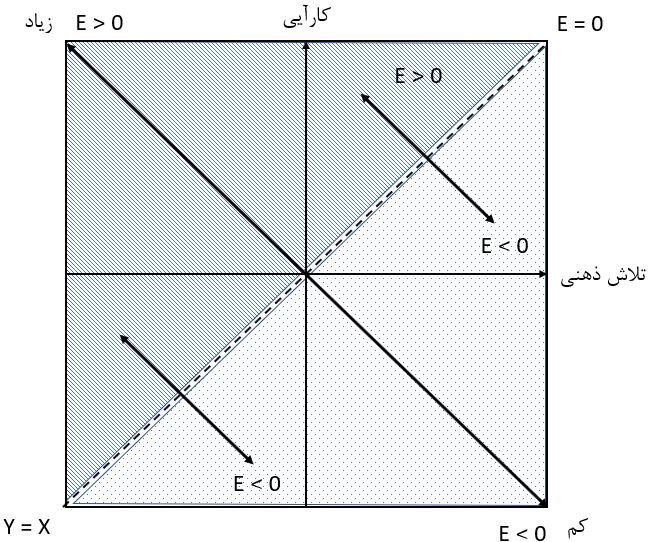
\includegraphics[width=0.7\linewidth]{figures/efficiency}
	\caption[بازنمایی گرافیکی کارآیی]{محور افقی نشان دهنده تلاش ذهنی و محور عمودی کارآیی خواهد بود، طبق شکل نواحی حاشور خورده دارای کارایی مثبت و نواحی نقطه‌ای دارای کارآیی منفی هستند.}
	\label{fig:efficiency}
\end{figure}

در یک بررسی دیگر توسط پاس و ون‌گوک از سال ۱۹۹۳ تا ۲۰۰۷ که بیش از ۳۰ مورد پژوهش در رابطه با نظریه‌ی بار شناختی را شامل می شد که از معیار کارآیی استفاده کرده بودند. با این حال همان طور که پاس و ونگوک اشاره کرده بودند تفاوت هایی بین روش امتیاز دهی ذهنی وجود داشت باعث ایجاد تفاوت‌هایی که در روش امتیاز دهی ذهنی وجود داشت باعث ایجاد تفاوت هایی در کارآیی شده است. زیرا كارآیی طبق  فرمول  به 
اندازهگيریهای ذهنی بستگی دارد. آنها اظهار داشتند كه رویکردهای گوناگون، انواع مختلف كارآیی ر ا 
می‌سنجد.  استفاده  از  امتياز های ذهنی  جمع آوری شده  پس از  آزمون،  عواقب  یادگيری ساخت
ساختارهای شناختی نظير الگوهای ذهنی را اندازهگيری می‌كند، درحالیكه اندازهگيریهای بعدی نشان
دهندهی كارآیی آموزش است.
\cite{van2008instructional}
\\
كارآیی یادگيری می‌تواند شاخص خوبی برای طراحی و خودكارسازی باشد. اگر دانش آموزان الگوهای
جدیدی به دست آورند و بتوانند با استفاده از آنها با تلاش كمتری یاد بگيرند، آن الگو قوی به حساب
می‌آید حتی اگر طراحی آموزشی بيشتری نياز باشد. با این وجود، بازدهی آموزشی نقش مهمی دارد، زیرا
نشان می‌دهد كه فرآیند یادگيری به چه شکل كارآمد است. دانستن ميزان سختی یا آسانی در طراحی
آموزشی، نقش مهمی در نظریهی بار شناختی دارد. با وجود این تفاوت در رویکردها، هر دو محاسبه كار آیی
آموزش و عملکرد در یادگيری اطلاعات در یک آزمون مهم هستند و می‌توانند اطلاعات حياتی مربوط به 
طراحی آموزشی را فراهم كنند.
\cite{sweller2011measuring}
\paragraph{مسائل مهم محاسبه‌ی کارآیی}
با وجود استفاده در مقياس وسيع، هافمن و شارو برخی از نگرانیهای مربوط به محاسبه كارآیی
آموزشی را شناسایی كردند. در بررسی كارآیی، آنها مدل اصلی پاس و ونمرینبور را به عنوان یک الگوی
انحراف
\LTRfootnote{Deviation model} 
دسته بندی كردهاند، زیرا بر اساس اختلاف بين نمر ههای عملکرد و تلاش استاندارد شده، 
محاسبه می‌شود. آنها استدلال كردند كه تفسير معنای تفریق دو متغير كه متفاوت از یکدیگر هستند ،
دشوار است. آنها این مثال را مطرح كردند كه مشابه این است كه هوش و وزن فرد را كه به صورت z-score
درآمدهاند را از هم كم كنيم. بنابراین تفسير نتيجهی نمرهی به دست آمده مشکل است.
\LTRfootnote{text}
\cite{hoffman2010conceptions}
آنها همچنين اشاره كردند كه اندازهگيری كارآیی تنها میتواند بر اساس دادههای گروهی باشد و در
نتيجه نمی‌تواند برای مقایسهی كارآیی فرد استفاده شود. از سوی دیگر آنها پيشنهاد كردند كه تفاوتهای
یافت شده در رفتار كلی مقایسه شود. بيشتر مطالعه‌های انجام شده در چارچوب نظریه‌ی بار شناختی به طور
كلی بر روی تفاوتهای گروهی تمركز می‌كنند، بنابراین مقایسه‌های فردی مسئله‌ای نيست. هافمن و شارو به عنوان جایگزینی برای مدل انحراف، مزایای دو روش دیگر را توصيف كردند: الگوی احتمال ،
\LTRfootnote{Likelihood model}
بر اساس 
نسبت عملکرد و امتيازدهی و الگوی احتمال شرطی ،
\LTRfootnote{Conditional likelihood model}
بر اساس نسبت احتمالها.
\cite{hoffman2010conceptions}
هافمن و شارو، مدل انحراف را  ضعيف نمی‌دانند بلکه مدعی هستند كه الگوهای مختلف با اهداف 
تحقيق مختلف ،متفاوت هستند. با این وجود، بر اساس تجزیه و تحليل هافمن و شارو محاسبهی نسبت 
عملکرد  و  امتيازدهی خودانگارانه (الگوی احتمال) بسيار ساده  است  و  می‌توانند برای تعيين اندازه‌ی
كارآیی فردی مورد استفاده قرار گيرند. این اندازهگيری‌های خودانگارانه می‌توانند به راحتی تركيب شود تا 
كارآیی گروهی را كه برای مقایسه‌ی رفتارهای كلی ضروری است فراهم كنند. انتظار می‌رود پژوهش‌های
آتی برای محاسبهی كارآیی، بيشتر از الگوهای احتمالاتی استفاده كنند.
\cite{hoffman2010conceptions}
\subsubsection{سنجش بارشناختی از طریق یک کار ثانویه}
معيارهای ذهنی كه  در  بالا  شرح  داده  شدند،  شایعترین ابزار  مورد استفاده  برای اندازهگيری بار 
شناختی بودند. با این حال، روش سنتی برای ارزیابی بار حافظهی كاری استفاده از كار ثانویه است كه با 
كار اصلی
\LTRfootnote{Primary task}
تركيب می‌شود (روش دوگانه) .یک كار ثانویه، مستلزم این است كه یادگيرنده علاوه بر كار 
اصلی یا حل مسئله، با فعاليت شناختی دیگری كه به كار اصلی اضافه می‌شود، درگير شود. برای مثال، در
حالی كه فرد در حال یادگيری چگونگی حل یک مجموعه مسائل ریاضی است، از وی خواسته می‌شود تا به 
نحو مشخصی به یک صدای خاص به عنوان یک فعاليت ثانویه پاسخ دهد. اگر كار اصلی بار شناختی
سنگينی را تحميل كند، عملکرد در كار ثانویه بدتر می‌شود. در مقابل، بار شناختی كمتر در كار اصلی
می‌تواند عملکرد بهبود یافته در كار ثانویه را افزایش دهد.
\cite{sweller1988cognitive}
\\
معمولا، كار ثانویه كاملا متفاوت با كار اصلی و نياز به منابع حافظه كمتر نسبت به كار اصلی دارد؛ با این
حال،  سویلر یک جایگزین برای این قالب ایجاد كرد.  سویلر معتقد  است  كه  درخواست  كردن  از  دانش
آموزان در حل مسئله از طریق یادگيری شامل دو فرآیند است:
\begin{enumerate}
	\item حل مسئله، كار اصلی
	\item یادگيری از 
	طریق تجربه، كار ثانویه.
\end{enumerate}
به عبارت دیگر، زمانی كه فراگيران در حال حل مسئله به عنوان وظيفهی اصلی
هستند، ممکن است این درگيری بر عملکرد كار ثانویه تأثير بگذارد. مشکل پيچيدهتر این است كه كمتر در 
مورد كار ثانویه یاد بگيرند. شواهد تجربی بر اساس یک كار خاص ثانویه كه شامل یادآوری دادهها و راه حل 
یک مشکل  پيشين است،  این استدلال  را  پشتيبانی  می‌كند.  فرآیندهای آموزشی در  جهت  كاهش  بار شناختی مرتبط با حل مسئلهای كه اطلاعاتی كه نياز به یادآوری برای حل مسئلهی قبلی دارد حركت 
می‌كند.
\cite{sweller1988cognitive}
\\
در یک استفاده  سنتی از  یک كار  ثانویه، ماركوس  و  همکاران  تعامل  با  عناصر  ارائهی آموزشی را 
موردبررسی قرار دادند و به طور خاص بررسی كردند كه یک نمودار چگونه تعامل با عناصر را  نسبت به 
حالتی كه فقط متن نمایش داده می‌شود، كم می‌كند. در این مطالعه، دو نوع كار ثانویه مورداستفاده قرار 
گرفت كه در هر دو، كار اصلی یکسان بود. در یک آزمایش، كار ثانویه این بود كه صدای بوق را كه به صورت 
تصادفی در طول یادگيری پخش می‌شود، تشخيص دهند. یادگيرندگان باید به محض شنيدن صدا، یک
پدال پایی را  فشار می‌دادند .زمان پاسخ
 \LTRfootnote{Response time}
به عنوان معياری برای اندازهگيری بار شناختی اعمال شده 
توسط كار اصلی، مورداستفاده قرار گرفت. در آزمایش دوم، كار ثانویه، یادآوری اعداد دو رقمی بود كه در 
حين كار اصلی به نمایش درمی‌آمدند. در این مورد، دقت یادآوری اعداد در كار ثانویه، به عنوان معياری
برای اندازهگيری بار شناختی استفاده شد. برای هر دو نوع كار ثانویه، نتایج قابل توجهی در تطابق با نتایج
یادگيری به دست آمد. استفاده از نمودارها و محتوای تعاملی كه منجر به نتایج بهتر، یادگيری و عملکرد
قویتر در وظایف ثانویه شد. از این رو در این پژوهش، توصيف بار شناختی مورد پشتيبانی قرار گرفت.
\cite{marcus1996understanding}
چندلر و سویلر نيز از یک روش دوگانه استفاده كردند تا نشان دهند كه كار ثانویه، كه یادآوری یک نشانه
بود، تحت تأثير قسمت آموزش قرار گرفته است. برای كار ثانویه، دو نشانهی جداگانه با صدای بوق  8ثانيه
بر روی صفحه نمایش كامپيوتر نمایش داده شد. یادگيرنده باید نشانهی اول را، در حالی كه نشانهی دوم را 
به خاطر می‌سپارد، به یاد آورد. نتایج نشان داد كه راهبرد آموزشی كه بار شناختی كمتری اعمال كند ،
دارای نمرههای بالاتری در كار ثانویه است. علاوه بر این، تفاوتهای قابل توجهی تنها برای راهبردهای
آموزشی و اقدام‌‌های ثانویه یافت شد، زمانی كه محتوای یادگيری دارای تعامل بالا با عناصر بودند. برای
محتوایی كه كمتر در تعامل با عناصر بودند، منابع حافظهی كاری بيشتری برای درگيری با كار ثانویه در 
دسترس بود، در نتيجه نتایج بهتری در آن به دست آمد و كمتر تحت تأثير قرار گرفت.
\cite{chandler1996cognitive}
در كارهای حل 
مسئله، در مقایسه با سایر وظایف، هالفورد، ميبری و باین
\cite{halford1986capacity}
و آیریس
\cite{ayres2001systematic}
از یک كار ثانویه استفاده
كردند تا نشان دهند كه تعامل بالا با عناصر، با بار حافظهی كاری بالا مطابق است.
\\
برونکن، اشتاینباخر، پلس و لوتنر از یادگيرندگان خواستند كه تغيير رنگ نشانههایی را كه در بالا ی
ارائه‌ی اصلی نمایش داده می‌شد ،رصد كنند. هنگامی كه رنگ تغيير كرد، یادگيرنده باید كليدی را كه روی
صفحه كليد مشخص شده است، فشار دهد. زمان پاسخ در این پژوهش، برای اندازهگيری بار شناختی استفاده شد. نتایج نشان دادند كه برای ارائههایی كه خوب طراحی شده بودند، بهترین عملکرد حاصل شد 
و دوباره از نظریهی بار شناختی پشتيبانی گردید.
\cite{brunken2004assessment}
\\
در پژوهش قبلی، كار ثانویه دیداری بود .در مطالعهی بعدی، برونکن ،پلس و لوتنر كار ثانویهی شنيداری
را موردبررسی قرار دادند. با استفاده از این استدلال كه محتوای شنيداری و دیداری در زیرسيستمهای
مختلف حافظه‌ی كاری پردازش می‌شوند، برونکن و همکاران معتقدند كه حالتهای مختلف (دیداری و 
شنيداری) كارهای ثانویه باعث بروز بار شناختی گوناگون در كانالهای مختلف حافظهی كاری خواهد شد.
به طور  خاص،  یک كار  ثانویه شنوایی باعث ایجاد تفاوتهای بار  شناختی در  كانال  شنوایی خواهد 
شد.
\cite{brunken2004assessment}
این فرض با استفاده از همان محتوای آموزشی كه برونکن و همکاران استفاده كردند انجام شد، 
با این تفاوت كه به جای رصد  كردن تغيير رنگ نشانهها، از صدای بوق كه به صورت تصادفی در طول 
آزمایش پخش  می‌شد، استفاده  كردند.  این بار  نيز از  زمان  پاسخ  به عنوان  معياری برای بار شناختی
استفاده گردید. همان طور كه پيشبينی می‌شد، كار ثانویهی شنيداری در مقایسه با كار ثانویهی دیداری،
موجب افزایش بار شناختی بيشتری در كانال شنوایی شد.
\cite{brunken2002assessment}
این دو مطالعه نشان دادند كه چگونگی
كار ثانویه عامل مهمی است كه باید در نظر گرفته شود.
\\
ون‌گرون، پاس، ونمرینبور و اشميت یک كار ثانویهی شنيداری-دیداری را موردبررسی قرار دادند. در 
این مطالعه، در  كار  ثانویه از  یادگيرندگان درخواست  شد  كه  روشنایی دكمهی یک نوع وسيلهی  پخش 
موسيقی
\LTRfootnote{Jukebox}
 را  كه  روبه‌روی محتوای آموزشی نشان داده  می‌شد، رصد  كنند. در این مطالعه  كار ثانویه‌ی
شنيداری-دیداری با كار ثانویهی تنها دیداری و تأثير سن موردبررسی قرار گرفت. نتایج یادگيری نشان داد 
كه افراد جوان بهتر از افراد مسن عمل كردند ولی اثری برای كيفيت محتوای آموزشی پيدا نشد. كار ثانویه،
این نتيجه را برگرداند: یادگيرندگان جوان، زمان پاسخ كمتری را نسبت به یادگيرندگان مسن داشتند. به
علاوه، اندازهگيری فردی بار شناختی نيز جمع آوری شد كه تفاوتهای ميان سن و كيفيت را نشان می‌داد .
جالب اینکه، حتی اگر هيچ اثری ناشی از كيفيت بر عملکرد آزمون وجود نداشت، اندازه‌گيری فردی،
ارائهی دوگانه  را  بهتر از  حالت ارائه‌ی واحد،  ارزیابی كرد.  این آزمایش نشان داد  كه  ارزیابی فردی، بار
شناختی را بهتر از كار ثانویه اندازه‌گيری می‌كند.
\cite{van2006modality}
\\
پژوهشها در حوزه نظریهی بار شناختی، كمتر از كار ثانویه نسبت به ارزیابی فردی به عنوان معياری
برای بار شناختی استفاده كردهاند. شاید سهولت استفاده دليل اصلی این تفاوت در استفاده از این دو 
روش باشد. ارزیابی فردی می‌تواند به سرعت و سادگی مورداستفاده قرار گيرد. این معيار را می‌توان برای
یک شخص یا تعدادی دانش آموز در یک كلاس، بدون امکانات خاصی به كار برد. در مقابل، كار ثانویه به برنامه ریزی بيشتری نياز دارد  و  بسته  به  طبيعت كار  ثانویه ممکن  است امکانات  خاصی نياز داشته 
باشد.
\cite{sweller2011measuring}
\\
با این وجود، مزیتهایی نيز در استفاده  از  كار ثانویه وجود  دار د.  مزیت اصلی این است كه  امکان
اندازهگيری بار شناختی پيوسته در طول یک كار فراهم است، در حالی كه ارزیابی فردی، بار سراسری
شناختی را پس از پایان كار اندازه‌گيری می‌كند.
\cite{sweller2011measuring}
\\
تاكنون اندازه‌گيری كارآیی با استفاده از كار ثانویه محاسبه نشده است. هيچ دليلی برای محاسبه نشدن
آنها وجود ندارد. تمامی معيارهای كارآیی كه توسط هافمن و شارو
\cite{hoffman2010conceptions}
بررسی شد می‌توانند به سادگی
توسط كار ثانویه به عنوان یک ارزیابی فردی محاسبه شوند، كه یک ارزش گذاری جدید برای بار شناختی
ایجاد می‌كند.
\subsubsection{سنجش فیزیولوژیکی بار شناختی}
% Chen, S., & Epps, J. (2013). Automatic classification of eye activity for cognitive load measurement with emotion interference.
چِن و اِپس
\cite{Chen2013}
با طبقه بندی داده‌هایی که توسط دستگاه ردیاب چشمی از کاربر گرفته‌ می‌شود توانستند معیار خوبی برای اندازه‌گیری بارشناختی به صورت هم‌زمان به‌دست آورند. از جمله ویژگی های اندازه گیری شده می‌توان به قطر‌ مردمک چشم، پلک زدن و حرکت‌های چشم اشاره کرد. آزمایش آن‌ها محاسبه‌‌های ریاضی و نشان دادن عکس به کاربر بود.
% pass

پاس و و نمرینبور یک معيار فردی را با تحليل نرخ ضربان قلب مقایسه كردند و نتيجه این بود كه معيار
فردی دارای پتانسيل بالاتری است.  تعداد  كمی از  مطالعات  فيزیولوژیکی پس از آن  توسط پژوهشگران 
نظریه‌ی بار شناختی در دهه‌ی بعد انجام شد. با این حال اخيرا، دوباره علاقه به این اقدامات ظهور كرده 
است.  واكنش  مردمکهای چشم
\LTRfootnote{Pupillary response}
به فعاليتهای شناختی، راهبرد دیگری بود  كه  امتحان شد.
\cite{paas1994variability}
ونگرون،  پاس، ونمرینبور و  اشميت با اشاره به  كار كاهنمن و بيتی
\cite{kahneman1966pupil}
،استدلال كردند كه  اندازه‌ی
مردمک  می‌تواند به  بار  حافظه‌ی كاری مربوط  باشد.  با  استفاده  از یک مجموعه تکاليف كه  نياز به  بار 
حافظهی مختلفی داشتند،  پيشنهاد كردند  كه  اندازهی مردمک  چشم،  با  افزایش بار حافظه، بيشتر
می‌شود. با این وجود یکی از محدودیت این معيار، سن فرد است زیرا با افزایش سن، همبستگی این معيار
با بارشناختی كم می‌شود و پاسخ قابل اعتمادی به دست نمی‌آید.
\cite{van2004memory}
پژوهشگران برای اندازهگيری بار شناختی از روشهایی مانند تصویرسازی تشدید مغناطيسی كاركردی
(اف‌ام‌آرآی)
\LTRfootnote{Functional Magnetic Resonance Imaging(FMRI)}
و الکتروانسفالوگرافی (ای‌ای‌جی) نيز استفاده  كرده‌اند.  این علاقه  همزمان  با  توسعه‌ی
فناوری‌های پيچيده‌تر بود.  شواهد نشان می‌دهد كه  روشهای فيزیولوژیکی می‌توانند شایستگی قابل
توجهی داشته باشد.
\cite{sweller2011measuring}
برای مثال، آنتوننکو و نایدرهاوسر هر دو مقياسهای فردی و ایایجی را در یک
مطالعه كه یادگيری را با استفاده از ابرمتن‌ها بررسی می‌كرد، جمع آوری كردند. تلاش ذهنی به عنوان 
مقياسی برای اندازه‌گيری فردی مورداستفاده قرار گرفت و ای‌ای‌جی از موج‌های آلفا، بتا و تتا جمع آوری شد. نتایج تحقيقات نشان داد كه استفاده از ابرمتن، نتایج یادگيری بهتری را در مقایسه با عدم استفاده از 
آن،  حاصل  كرد.  در حالی كه هيچ تفاوتی بين گروهی، برای اندازه‌گيری تلاش  ذهنی یافت نشد،
اندازه‌گيری‌های آلفا، بتا و تتا در گروهی كه از ابرمتن استفاده می‌كردند به طور قابل توجهی كم بود. نتيجه
این بود كه ابرمتن موجب كاهش بار شناختی می‌شود و تنها ای‌ای‌جی به اندازه‌ی كافی، حساس به این
تفاوت‌ها بود.  درباره‌ی شکست  روش  فردی، آنتوننکو  و  نایدرهاوسر استدلال  كردند  كه  مزیت روش 
ایایجی این بود كه سطوح مختلفی از بار را بازتاب میدهد، مانند بار لحظه‌ای، بار بيشينه، بار ميانگين،
بار تجمعی و  بار  سراسری. در حالی كه اندازه‌گيری فردی تنها  می‌تواند بار سراسری را  اندازه‌گيری
كند.
\cite{antonenko2010influence}
در یک پژوهش، روشه‌ای برخط 
\LTRfootnote{Online}
مانند رهگيری چشم و رصد ضربان قلب 
\LTRfootnote{Heart rate}
كه می‌تواند در طول
یادگيری و آزمون استفاده شوند و روشهای برون خط 
\LTRfootnote{Offline}
مانند اندازهگيریهای فردی كه تنها بعد از اتمام 
فعاليت میتوان آنها را به كار گرفت، تمایز قائل شدند. در طی چند سال گذشته، پژوهشها درزمينهی
نظریهی بار شناختی و محيطهای آموزش چندرسانهای، برای ردیابی بيشتر از ر هگيری چشم  استفاده 
كردهاند. بعضی شواهد نيز نشان دادهاند كه می‌توان از رهگيری چشم برای اندازه‌گيری نوسان‌های بار 
شناختی استفاده  كرد.  پژوهشگران  دریافتند كه  تركيبهای مختلف متن و  تصویر كه  نيازمند سطوح 
مختلفی از پردازش شناختی هستند، با تغييرهای تثبيت‌های چشمی 
\LTRfootnote{Eye fixations}
همبستگی داشتند. به طور كلی
نشان داده شده است كه تثبيت طولانیتر چشم، نشاندهندهی پردازش شناختی بيشتر است. در نتيجه،
دادههای رهگيری چشم دارای شایستگی قابل توجهی هستند، زیرا نه تنها نشان میدهند كه یادگيرنده به 
كجا تمركز می‌كند، بلکه مدت توجه وی را نيز رصد می‌نماید كه متناظر با تغييرهای بار شناختی است.
\cite{sweller2011measuring}
یکی دیگر از راهبردهای برخط كه برای استفاده دارای قابليت است، به كارگيری شاخصهای پيچيدگی
زبان است. در حالی كه این معيار ذاتا فيزیولوژیکی نيست، پيچيدگی گفتاری بسياری از مشخصههای
معيارهای فيزیولوژیکی را به اشتراک می‌گذارد كه شامل قابليت استفادهی برخط است و به طور همزمان با 
یادگيری و آزمون قابل به كارگيری است.
\cite{sweller2011measuring}
خواجه، چن و ماركوس معتقدند كه با افزایش دشواری كار، 
چگالی واژگان بيان، كاهش می‌یابد. این اثر در یک مطالعه بر روی گروههای مدیریت حوادث آتش سوزی
جنگل  گزارش  شده  است.  هر چقدر  كه آتش سوزی چالشانگيزتر و  شامل  حوادث  غيرمنتظره بود، 
الگوهای گفتاری گروههای عملياتی تغيير یافت و با توجه به پيچيدگیهای كاری دارای چگالی كمتری شد. از این رو، اندازهگيری پيچيدگی زبان به صورت بالقوه یکی دیگر از شاخصهای مفيد برخط برای بار 
شناختی است.
\cite{khawaja2010using}
در حال حاضر، بعد از آغازی نااميدكننده، شاخصهای فيزیولوژیکی سرانجام به عنوان جایگزینهای
مناسبی برای روشهای فردی، جزو علاقه‌مندیهای پژوهشگران است. برخی از روشها اميدواركننده
هستند، اما هنوز هم خيلی زود است كه با وجود تأكيد پژوهشها بر این روشها، آنها را جامع بدانيم. در 
گذشته نشان داده  شده  است كه استفاده از روشهای فيزیولوژیکی، نسبت به تفاوتهای بار شناختی
توليدشده توسط طراحیهای آموزشی مختلف به صورت كافی حساس نبوده است. هنوز مشخص نشده 
است  كه  آیا تلاشهای كنونی برای یافتن اقدامات  فيزیولوژیکی كه  به  اندازهی  كافی حساس  باشند،
موفقيت آميز خواهد  بود  یا نه.
\cite{sweller2011measuring}
در  فصل  بعد  به  صورت  خاص،  به  بررسی  دو  روش  پراستفادهی 
فيزیولوژیکی چشمی (رهگيری چشم) و مغزی (ای‌ای‌جی) برای سنجش بار شناختی  در فرآیند یادگيری
چندرسانه‌ای از طریق فيلم آموزشی می‌پردازیم.

\subsubsection{سنجش انواع مختلف بار شناختی}
پس  از  شناسایی دسته‌های  مختلف  از  بار  شناختی، پيشبينیهای نظری بر  اساس  بار  شناختی
پيچيدهتر شد. پژوهشگران به جای استفاده از بار شناختی سراسری برای استدلال اینکه چرا یک طراحی
آموزشی كارآمد است یا نه، شروع به تفکيک بين دستههای بار شناختی برای صورت بندی فرضيههای خود 
كردند. از این رو در دهه گذشته علاقهی زیادی برای دستيابی به روشهایی بر ای اندازهگيری انواع مختلف 
بار شناختی به وجود آمده است.
\cite{antonenko2010using}
\\
از لحاظ نظری، فرض بر این است كه بار شناختی ذاتی و فرعی به كل بار شناختی افزوده می‌شود.
موضوع سادهای است كه بار شناختی ذاتی و فرعی را بهوسيلهی روشهای تجربی متمایز كنيم. در یک
آزمایش آموزشی، اگر بار شناختی ذاتی ثابت نگه داشته شود و بار شناختی فرعی در آزمایشها فرق داشته 
باشد،  این اختلاف  باید در  نتایج اندازهگيریهای فردی نيز مشاهده  شود  كه  این تفاوتها نمایانگر بار 
شناختی فرعی است. به طور مشابه، با ثابت نگهداشتن بار فرعی و متغير كردن بار ذاتی می‌توان با استفاده 
از ميزان تفاوت‌ها در اندازه‌گيری‌ها، بار ذاتی را نيز محاسبه كرد. آیریس از این قانون به عنوان اولين تلاش 
برای اندازه‌گيری بار شناختی ذاتی استفاده كرد.
\cite{antonenko2010using}
\\
با استفاده از یک تکليف حل مسئله، آیریس از دانش آموزان خواست تا مجموعهای از مسئلههای جبری
را كه نياز به محاسبه‌های پی در پی دارند ،حل كنند. چون دانش آموزان قبلا دربارهی این مسئله آموزش دیده
بودند، آیریس استدلال كرد كه بار فرعی مطابق با فاكتورهای آموزشی ثابت است.
\cite{ayres2006using}
در مطالعهی قبلی، آیریس دریافت كه دانش آموزان با توجه به محل محاسبه‌ها، خطاهای نمایه‌ای 
\LTRfootnote{Error profiles}
خاصی را نمایش دادند. 
بعضی از  محاسبه‌ها،  بيشتر نيازمند تعامل بودند  و  در نتيجه نرخ  خطای بالاتری در  آن  نقاط  مشاهده 
شد.
\cite{ayres2001systematic}
آیریس از دانش آموزان خواست كه به محض حل مسئله ،ميزان آسانی یا دشواری را كه در طول 
هر مرحله از حل مسئله تجربه كردند، امتيازدهی كنند. نتایج، تطابق پایداری را بين امتيازدهی دشواری و 
الگوهای خطا نشان داد. از طریق امتيازدهی فردی برای هر مرحله از مسئله، این امکان فراهم شد كه 
تعامل با عناصر (بار شناختی ذاتی) داخل هر مسئله نيز قابل محاسبه باشد. همچنين دانش آموزانی كه
دارای دامنهی دانش بيشتری بودند، از طریق امتيازدهی فردیشان، راحت‌تر می‌شد آنها  را  از دانش
آموزانی كه دانش قبلی كمتری داشتند،  متمایز كرد.  آنهایی كه احتمالا بيشترین دانش  را  داشتند، 
امتيازدهی را با دقت و عمق بيشتری انجام دادند. حتی اگر دانش آموزان با توانایی بالا، خطاهای اندكی را 
انجام دهند، باز هم قادر بودند تفاوت ميان عناصر تعاملی را در سطوح مختلف شناسایی كنند. در این
مطالعه، هيچ تلاشی برای ارائهی مباحث جداگانهای از دستههای مختلف بار شناختی انجام نشده است. 
در عوض، بار شناختی فرعی ثابت نگه داشته شد و در نتيجه هرگونه تفاوت بار ممکن است به خاطر بار 
ذاتی باشد.
\cite{ayres2006using}
\\
دیليو و مایر از رویکرد تركيبی متشکل از معيارهای ذهنی و یک كار ثانوی برای بررسی اینکه آیا ابزارهای
مختلف می‌توانند بار شناختی ذاتی، فرعی و وابسته را جداگانه اندازهگيری كنند، استفاده كردند. دیليو و 
مایر استدلال می‌كنند كه  بار  ذاتی را  می‌توان با  افزایش تعداد  جملههای توضيحی در  یک درس 
چندرسانهای و بار اضافی را با تغيير محتوای اضافی متشکل از همان متن و گفتار دستكاری كرد. عملکرد 
در هنگام انتقال مطالب معياری برای اندازهگيری بار شناختی وابسته بود. سه معيار بار شناختی جمعآوری
شد :زمان پاسخ به فعاليت ثانویه كه شامل تغيير رنگ پسزمينه بود، امتيازدهی فردی تلاش ذهنی در طول 
درس و امتيازدهی ميزان دشواری كه بعد از درس جمعآوری شد. در دو آزمایش، مشخص شد كه كار ثانویه
بيشترین حساسيت را  به دستكاری افزونگی (بار فرعی )داشت، تلاش ذهنی بيش از همه به تغييرهای
پيچيدگی جمله‌ها (بار  ذاتی) حساس  بود،  و  امتيازدهی دشواری نيز بيشترین حساسيت را  به  ميزان
موفقيت در انتقال مطالب داشت. دانش آموزانی كه بالاترین نمرهها را به چگونگی انتقال مطالب دادند
تلاش  وابستهی بيشتری داشتند  و  كسانی كه  نمرههای پایين را  دادند  تلاش  وابستهی كمتری انجام 
دادند.
\cite{deleeuw2008comparison}
\\
این یافته‌ها نشان  می‌دهد كه  اندازه‌گيری‌های مختلف  می‌تواند به  فرآیندهای مختلف  ضربه  بزند  و 
حساسيت‌های مختلف را نشان دهند. با این وجود، ممکن است شک داشته باشيد كه آیا سه روش استفاده شده می‌توانند انواع مختلف بار شناختی را تشخيص دهند یا خير. روشن نيست كه چرا  یک كار ثانویه
نسبت به بار شناختی فرعی باید بيشتر از تلاش ذهنی حساس باشد یا چرا تلاش ذهنی باید به طور خاص 
بر روی بار ذاتی حساس باشد. علاوه بر این، شک برانگيز است كه عملکرد انتقال لزوما یک معيار برای
اندازهگيری بار وابسته باشد. افزون بر این، باید توجه كرد كه با توجه به صورت بندی فعلی، بار شناختی
وابسته صرفا انعکاسی از مقدار بار اعمال شده توسط عناصر تعاملی ذاتی است و بنابراین به طور مستقل به 
بار كل كمک نمی‌كند. با این وجود جالب است كه این اندازه‌گيری مختلف بر اساس ماهيت دستكاری‌ها
است. مطالعه‌های بسيار كمی از هر دو معيار امتياز دهی خودانگارانه و مقياس كار ثانویه برای اندازهگيری
بار شناختی، استفاده كردهاند.
\cite{antonenko2010using}
\\
\paragraph{شاخص بار کاری ناسا}
در تلاش برای اندازه‌گيری جنبه‌های مختلف بار شناختی، برخی از پژوهشگران تحت تأثير یک مقياس
چندبعدی به نام شاخص بار كاری ناسا 
\LTRfootnote{NASA Task Load Index (NASA-TLX)}
قرار گرفتند.
\cite{hart1988development}
این شاخص، شامل شش زیرمقياس است كه 
عوامل مختلفی را  در رابطه با تکميل یک كار، اندازه‌گيری می‌كند :
\begin{enumerate}
	\item نيازمندیهای ذهنی
	\LTRfootnote{Mental demands}
	 چقدر 
	فعاليت ذهنی و  ادراكی موردنياز بود؟
	\item نيازمندیهای فيزیکی 
	\LTRfootnote{Physical demands}
	چقدر  فعاليت فيزیکی موردنياز
	بود؟
	\item نيازمندیهای زمانی 
	\LTRfootnote{Temporal demands}
	چقدر فشار زمان رخ داده است؟
	\item كارآیی به نظر شما، موفقيت
	شما در انجام اهداف تعيين شده توسط آزمایشگر چقدر بوده است؟
	\item تلاش چقدر دشوار بود كه با 
	انجام كار ذهنی و فيزیکی به سطح كارآیی مورد انتظار خود برسيد؟
	\item سطح نااميدی 
	\LTRfootnote{Frustration}
	چقدر در طول 
	انجام این كار، احساس ناامنی، نااميدی، عصبی شدن، پریشانی را  به جای احساس امنيت، رضایت و 
	آرامش تجربه كردید؟ 
\end{enumerate}
از طریق تركيب این زیرمقياس‌ها یک اندازه‌گيری سراسری از بار ذهنی محاسبه 
می‌شود.
\cite{antonenko2010using}
\\
\begin{figure}[htbp]
	\centering
	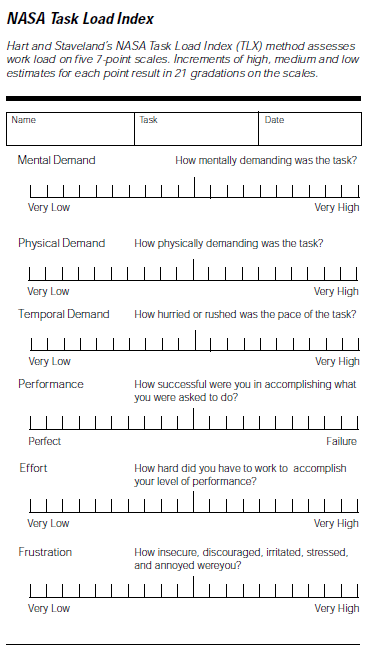
\includegraphics[width=0.7\linewidth]{figures/NasaTLX}
	\caption[پرسش نامه‌ی شاخص بار کاری ناسا]{نمونه‌ی معیار پرسش‌نامه‌ی شاخص بار کاری ناسا}
	\label{fig:nasatlx}
\end{figure}

اخيرا در یک بازتاب از استفاده از این شاخص، هارت متوجه شد كه این مقياس عمدتا در مطالعه‌هایی كه 
بر روی طراحی واسط  و  ارزیابیها متمركز  بودند، استفاده  شده  است  كه  شامل  تأثير خودكارسازی و 
تصميمگيری بودند.
\cite{hart2006nasa}
\\
علاوه بر این، مطابق با اهداف اصلی كه برای آن طراحی شده، در بسياری از مطالعه‌ها كنترل ترافيک
هوایی و سایر فعاليتهای هوافضایی استفاده شده است. در مقابل، پژوهشگران نظریهی بار شناختی كه 
روی محيط یادگيری متمركز شده بودند و از این مقياس استفاده كردند، اغلب ساختار آن را با انتخاب 
بعضی زیرمقياسها تغيير دادند .همچنين صورت برخی از سوالها را نيز عوض كردند.
\cite{antonenko2010using}
در تلاش برای
اندازه‌گيری دسته‌های مختلف بار شناختی، شایتر، گرجتز ،و كاتامبن سه مورد از سوال‌ها را انتخاب كردند:
«نيازمندی‌های كار( »
\LTRfootnote{Task demands}
مقدار فعاليت ذهنی و فيزیکی برای انجام تکليف یادگيری نياز بود؟) ،«تلاش» (به 
چه ميزان تلاش و كار نياز بود تا دانش آموز مفاهيم درس را متوجه شود؟) و «نيازمندیهای هدایت»
\LTRfootnote{Navigation demands}
)شركت كننده باید به چه ميزان تلاش كند تا محيط آموزش را كنترل كند؟). گرجتز و همکاران استدلال 
كردند كه هركدام از این موارد می‌تواند به ترتيب ،متناظر با بار شناختی ذاتی، وابسته و فرعی باشد. نتایجی
از یک مطالعه كه پيچيدگی مثال‌های كار شده را دستكاری می‌كرد نشان داد كه موافقت گسترده‌ای با 
داده‌های عملکرد وجود دارد. به عبارت دیگر، گروه‌هایی با بالاترین ميزان یادگيری، كمترین ميزان بار 
شناختی را گزارش كردند. با این حال، شواهدی برای مشاركت این سه معيار با انواع مختلف بار شناختی
ذكرشده ،وجود ندارد.
\cite{gerjets2006can}
\\
\paragraph{اصل حجم‌کاری ورودی ترافیک هوایی}
این اصل که به اختصار 
ATWIT
\LTRfootnote{Air Traffic Workload Input Technique}
خوانده می‌شود، اولین بار توسط استین معرفی شد.
\cite{stein1985air}
این معیار در مقایسه با معیار ناسا که تنها می‌تواند در انتهای فعالیت شناختی استفاده شود، آزدی بیشتری دارد و این اجازه را می‌دهد تا در حین فرآیند یادگیری از آن استفاده شود. این معیار برای سیستم‌ها و مطالعه‌های کنترل ترافیک هوایی طراحی شده با این حال در حوزه های دیگر نیز مورد بررسی قرار گرفته و عملکرد آن ثابت شده است. در این روش از یک مقیاس ۱( حجم‌کاری کم) تا ۷ (حجم کاری زیاد) نمره‌ای استفاده می‌شود که در این حین فرآیند یادگیری کاملا متوقف شده و از یادگیرنده خواسته می‌شود تا بار کاری خود را گزارش کند. یکی از مزیت های استفاده از این روش آن است که به ما اجازه می‌دهد تا ارزیابی دقیق تری در حین آزمایش شناختی داشته باشیم، به جای آنکه تا انتهای آزمایش صبر کنیم و بار شناختی را گزارش دهیم. در تصویر
\ref{fig:atwit}
نمونه‌ای از این پرسشنامه را می‌بینید.

\begin{figure}[htbp]
	\centering
	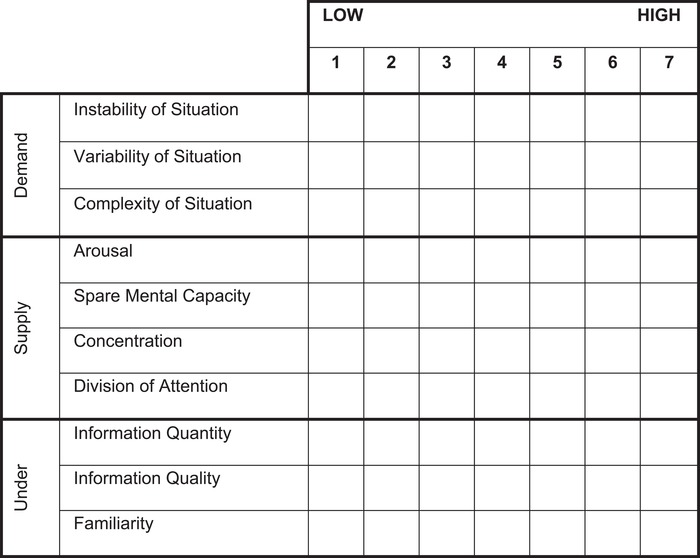
\includegraphics[width=0.7\linewidth]{figures/ATWIT}
	\caption[پرسش نامه‌ی ترافیک‌هوایی]{در پرسشنامه حجم‌کاری ترافیک هوایی مقیاس ها از ۱ تا ۷ هستند. و می‌توان در طول فرآیند آزمایش از یادگیرنده گرفته شود.}
	\label{fig:atwit}
\end{figure}

در جستجوی معيارهای متفاوت‌تری برای بار شناختی، تمایل به اصلاح جمله‌های پرسش‌نامه به نحوی كه
با  انواع مختلف  بار  شناختی متناظر  باشند، به  وجود  آمد.  برای برخی از  پژوهشگران  از  مواردی مانند
«محتوای آموزشی برای شما چقدر دشوار بود؟ چقدر برایتان مشکل بود تا مفاهيم را یاد بگيرید؟ چقدر در 
طول یادگيری تمركز داشتهاید؟» استفاده كردند. دليل این جمله بندی برقراری ارتباط با سه سطح مختلف 
بار شناختی بود. سؤال اول مربوط به بار ذاتی، سؤال دوم مربوط به بار فرعی و سؤال سوم نيز در رابطه با بار 
وابسته است. در این مطالعه، بين اندازهگيریهای شناختی بار و دادههای كارآیی، ارتباط قابل توجهی
یافت شد. با این حال، گاهی وقت‌ها  ارتباط‌های بين آزمون  كارآیی و  اندازه‌گيری‌های بار  شناختی با 
پيشبينی‌های نظری تطابق ندارد. در تعدادی از مطالعه‌ها جمله بندی‌های با تنوع بيشتری را به كار بر دند. 
از دانش آموزان خواسته شد تا به «دشواری دامنه» (بار ذاتی) و «چقدر تلاش برای درک مفاهيم مثالها 
انجام  دادید؟» (بار وابسته) امتيازدهی كنند.  با این حال، این مطالعه  ارتباط  مورد  انتظار  بين
اندازهگيریهای بار شناختی و نتایج یادگيری را نيافت.
\cite{sweller2011measuring}
\\
ناسازگاریهای فوق در تلاشهای روانسنجی برای اندازهگيری انواع مختلف بار شناختی غيرمنتظره
نيست. تمایزهای روانشناسانه بين دستههای مختلف بار شناختی نياز به این دارد كه یادگيرندگان نشان 
دهند كه به چه ميزان از هر دستهی بار شناختی متحمل شدند. ما به یادگيرندگان شک داریم، به خصوص 
یادگيرندگان تازه وارد قادر به ایجاد تمایز موردنياز نيستند.
\cite{sweller2011measuring}
\\
% 4- Measurement with Eye and EEG
\section{معیار‌های داده‌های چشمی و مغزی و ویژگی‌های آن‌ها}
\label{s:eye}
\subsection{مقدمه}
در بخش
\ref{s:CognitiveLoad}
دیدیم معیار های اندازه گیری شناختی را می‌توان به دو صورت دسته بندی نمود، نخست واقعیت گرانه 
\LTRfootnote{Objective}
و خود انگارانه یا مستقیم و غیرمستقیم. با این حال سنجش واقعیت گرایانه بارشناختی در میان پژوهش‌ها کمتر بوده‌ است. سنجش با فعالیت ثانویه که شامل یک فعالیت دیگر بودند و بار شناختی اعمال شده توسط فعالیت اصلی را با کارایی و یا زمان پاسخ فعالیت ثانویه اندازه‌گیری می‌شوند. سنجش با فعالیت ثانویه نمی‌تواند به صورت پیوسته بار شناختی را اندازه گیری نماید، با این‌حال می‌توان  زمان پاسخ دادن به فعالیت ثانویه را در بازه اعمال و یا نمایش محرک فعالیت ثانویه استناد نمود.
\cite{antonenko2010using}
\\
حال روش هایی مانند رهگیری چشمی و ای‌ای‌جی که در سال های گذشته عمدتاً در شرایط آزمایشی ویژه و محدود به کار می‌رفتند، اكنون به طور فزاینده در محيطهای یادگيری واقع گرایانه كاربرد دارد. قابليت این 
روشها برای پایش و سنجش آنی و كمی وضعيت شناختی و ذهنی یادگيرندگان، می‌تواند استفاده زیادی 
در بهينه سازی راهبردهای آموزشی داشته باشد.
\cite{jraidi2019assessing}
در این فصل، به بررسی سنجش بار شناختی با روش رهیاب چشمی در فرآیند یادگيری چندرسانهای از طریق فيلم آموزشی می‌پردازیم. 
همچنين جدیدترین پژوهشهای كاربردی این حوزه كه با كمک معيارهای چشمی به سنجش بار 
شناختی و یادگيری چندرسانه‌ای پرداخته‌اند، گزارش می‌كنيم.

سنجش پیوسته بارشناختی اجازه تحلیل دقیق تر میزان نوسان بارشناختی را با داشتن داده های زمان های مختلف به ما می‌دهد، بدین صورت می‌توان تحلیل و نتیجه‌گیری های دقیق تری از داده های بارشناختی و ارتباط آن با اثر انواع محرک های یادگیری داشت. روش های اندازه گیری واقعیت گرانه‌ی بار شناختی به ما این امکان را می‌دهند تا در تمامی سطوح شناختی شامل آنی، بیشینه، تجمعی، میانگین و سراسری بتوانیم بارشناختی را مورد بررسی قرار دهیم. از جمله این روش‌ها می‌توان به روش های سنجش  فیزیولوژیکی مانند: نرخ ضربان قلب
\LTRfootnote{Heart Rate Variability}
، حرکت چشم
\LTRfootnote{Eye Movements}
، سطح هرمون‌ها
\LTRfootnote{Hormone Levels}
و نوروآدرنالین
\LTRfootnote{Noradrenaline}.
و از جمله روش‌هایی که در علوم اعصاب استفاده شده‌اند، می‌توان به تصویرسازی تشدید مغناطیسی کارکردی (اف‌ام‌آرآی)
\LTRfootnote{Functional Magnetic Resonance Imaging(FMRI)}
، برش‌نگاری با گسیل پوزیترون (پِت اسکن)
\LTRfootnote{Positron Emission Tomography(PET)}
و نوار مغزی (ای‌ای‌جی)
\LTRfootnote{Electroencephalography(EEG)}
اشاره نمود.
\cite{antonenko2010using}
\\
به عنوان گزینه‌ای برای اندازه گیری بار شناختی هریک محدودیت های خود را نیز دارند، برخی ارتباط ضعیف تری با بار شناختی برقرار می‌کنند(مانند نرخ پلک زدن، مدت پلک زدن). روش سطح هرمون‌ها سرعت بسیار کمی دارد، نرخ ضربان قلب به نوسان‌های لحظه‌ای بار شناختی حساس نمی‌باشد. برخی اندازه گیری ها نیز بیش از حد دست و پا گیر و مزاحم هستند و یا نیاز به کاربر متخصص که به دو حیطه شناختی و پزشکی آشنا باشد دارند مانند پست اسکن و اف‌ام‌آرآی در این روش ها تصویر برداری عصبی با استفاده از پویش‌گرها و حس‌گرها تغییرها‌را در جریان خون مرتبط با فعالیت عصبی را ثبت می‌کنند. در یک پژوهش مشاهده شده است که انقباض مردمک که هیچ‌یک از این محدودیت‌ها را ندارد برای فعالیت هایی که شامل خواندن پیوسته باشد مناسب نیست. همچنین علائمی وجود دارد که پاسخ مردمک به تغییرهای بار شناختی بسته به سن شرکت کنندگان کاهش می‌یابد.
\cite{antonenko2010using}
\\
در شکل 
\ref{fig:neuromarketingtools}
می‌توانید روش های مختلف بررسی فعالیت های مغزی را مشاهده کنید.
\begin{figure}[htbp]
	\centering
	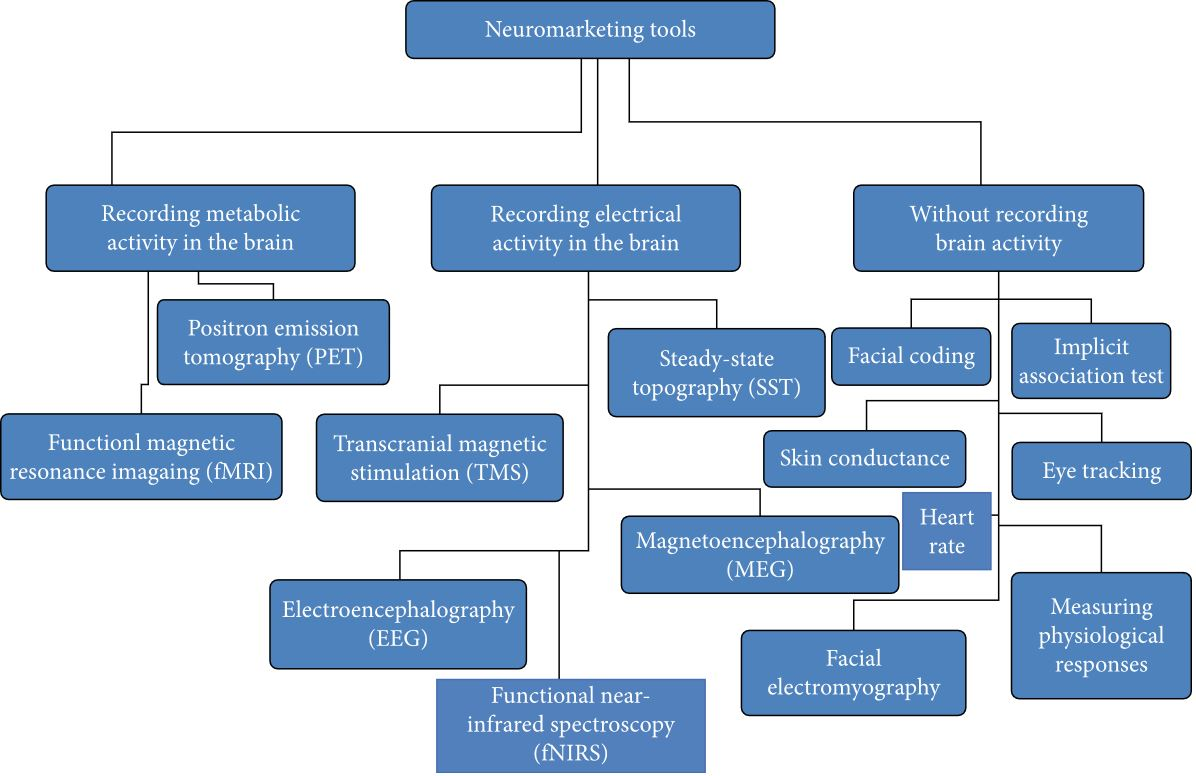
\includegraphics[width=\linewidth]{figures/Neuromarketing_tools}
	\caption[نمودار درختی روش‌های اندازه‌گیری بارشناختی]{نمودار درختی روش‌های اندازه گیری بارشناختی}
	\label{fig:neuromarketingtools}
\end{figure}


\subsection{پیشینه پژوهش های استفاده از ردیابی چشم}

نخست در سال ۱۸۷۹ لویس جوال مشاهده نمود که فرایند خواندن متن و حرکت چشم بر روی نوشته‌ها به صورت پیوسته و روان نیست، و در مکان های خاصی چشم متوقف (تثبیت چشم)و یا حرکت ناگهانی(پرش چشم) دارد.
با این مشاهده سوال های جالبی در قرن بیستم میلادی بررسی شدند،‌از جمله چشم بر روی چه کلمه‌‌هایی توقف می‌کند؟ ، به چه مدت؟ و چه زمانی چشم به کلمه ای که قبلا دیده است باز می‌گردد.
\\
نخستین دستگاه ردیابی چشمی توسط ادموند هوی ساخته شد، نوعی  لنز بود که با چشم در تماس بود و یک درچه برای مردمک چشم روی آن تعبیه شده بود. که این لنز به نشانه گر آلومنیومی کوچکی متصل بود، او با این دستگاه به بررسی بازگشت چشم بر روی کلمه‌ها پرداخت و نشان داد که چشم روی برخی کلمه توقف نمی‌کند.
اولین دستگاهی که مزاحمتی برای چشم ایجاد نمی‌کرد توسط گای توماس باس‌ول، ساخته شده، که پرتوهای نوری که به چشم تابیده می‌شد را بر روی فیلم ذخیره می‌نمود. آلفرد یاربوس در کتابی که در ۱۹۶۷ میلادی منتشر کرد پژوهش های مهمی را بیان کرد و به طور خاص به رابطه تثبیت چشم و علاقه پرداخته بود.
در طول دهه ۱۹۸۰ جاست و کارپنتر فرضیه مهمی را بیان کردند که می‌گفت هر جا که چشم بر روی آن متوقف شده است ما در حال فکر کردن به آن هستیم و هرچه مدت زمان تثبیت بیشتر باشد بار شناختی بیشتری ایجاد شده است.
همچنین آغاز پاسخ دهی به سوال های رابطه انسان-رایانه بود.
در پژوهش های اخیر به رابطه میان انسان و کامپیوتر و استفاده از چشم برای تهسیل آن و آنالیز صفحه‌های وب پرداخته شده.
\\
به گفته هفامن توجه بینایی همیشه در حدود ۱۰۰ تا ۲۵۰ میلی ثانیه جلو تر از حرکت چشم قرار دارد و هر جا که توجه بینایی ما می‌رود چشم هم دنبال می‌کند.
\cite{deubel1996saccade}
به لطف پیشرفت فناوری و علم اکنون ردیابی های چشمی همراهی که بر روی چشم استفاده می‌شوند ساخته و تجاری سازی شده است، و دانش شبکه های عصبی عمیق
\LTRfootnote{Deep Learning Neural Network}
به ما کمک می‌کند تا بتوانیم این داده های چشمی را بهتر از گذشته پردازش کنیم.
\cite{wiki:EYET}
\subsection{مزیت‌ها و محدودیت‌ها‌ی اندازه گیری بار شناختی با استفاده از رهیاب چشمی}
\label{ss:ProVsCon}

برخلاف سایر دستگاههای فیزیولوژیکی که نیازمند دراز کشیدن شخص‌ در وضعیت محصور است (اف‌ام‌آرآی) یا خوردن مواد خطرناک(پِت‌اسکن)، ای‌ای‌جی بدون ورود به بدن می‌تواند فعالیتهای مغزی را به‌صورت‌ معتبر و با تنظیم‌های دنیای واقعی
\LTRfootnote{Real-World}
اندازه‌گیری کند.
\\
پیش از این فعالیت های مغزی با روش هایی چون نوار مغزی و مگنتوانسفالوگرافی یا به اختصار MEG
\LTRfootnote{Magnetoencephalography}
تهیه می‌شد. هدف این گونه ابزار ها رصد تغییر‌های میدان های مغناطیسی ایجاد شده در جمجمه توسط تغییر‌های جریان در نورون های مغزی بود.
بار شناختی یکی از شاخصه های فعالیت مغز است. عمده محبوبیت این روش ها دقت آن‌ها در حدود میلی ثانیه است، با اینحال عموما تنظیم آن آسان نیست و محاسبه‌های آن پیچیده تر است. همچنین نمی‌توان از داده های آن به صورت همزمان استفاده نمود و محل استفاده از آنها نمی‌تواند مکان های عمومی و یا حتی در مکان های عادی باشد.
\\
روش های بسیار غیر نورونی دیگری وجود دارد که نشان دهنده فعالیت های مغز و بار شناختی است. فعالیت های قشر بیرونی مغز سبب ایجاد تغییرهایی در ضربان قلب، فشار خون، الکترودرمال یا به اختصار EDA
\LTRfootnote{Electrodermal Activity}
، فعالیت های الکتریکی در عضله‌‌های صورت، حرکت‌های چشم و گشودگی مردک چشم.
\\
پژوهش های اخیر بر روی حرکت مردمک چشم جهت اندازه گیری بار شناختی سرمایه گذاری کرده‌اند.
تا کنون پژوهش های زیادی بر رابطه‌ی بین حرکت‌های ارادی چشم مانند توقف یا تثبیت چشم و پرش چشم با بارشناختی و یا حرک‌ت‌های غیر ارادی مثل پلک زدن و گشادی مردمک. به این حرکت‌های چشم رفتاری(ارادی) و فیزیکی(غیر ارادی) نیز گفته می‌شود.
با دنبال کردن حرکت‌های چشمی می‌توان به بررسی واکنش فیزیکی افراد نسبت به آزمایش  و سیستم می‌توان واسط کاربری متناسب با آن طراحی نمود.
به عنوان مثال در شرایط کنترل شده، رهیاب های چشمی با دقت بالا و مردمک سنج‌ها می‌توانند برای شناسایی کوچکترین گشودگی در مردمک استفاده شوند که نشانه بار شناختی است.
\cite{rafiqi2015pupilware}
با این حال باید توجه شود که سیستم های نمایش اطلاعات محتوی های بسیاری را نشان می‌دهند، نمایش اطلاعات و تعامل کاربر با سیستم تنوع بسیاری دارند که این خود سبب سخت شدن در استفاده مستقیم از حرکت‌های چشم در سنجش بار شناختی در مکان های عادی می‌شود. از این رو مهم است که رابطی بین حرکت‌های چشم و بار شناختی پیدا شود.
\cite{zagermann2016measuring}
\\
\textbf{تعامل انسان و رایانه}
\LTRfootnote{human computer interaction - HCI}
 به دانش و فناوری مدرن و پرتنوع مطالعه، طراحی، اجراء، و ارزیابی سامانه‌های محاسباتی درگیر در محاوره‌ها و تعامل‌های مابین کاربران انسانی از یک سو، و رایانه‌ها و عامل‌های هوشمند نرم‌افزاری از سوی دیگر گفته می‌شود. این دانش به بررسی تعامل انسان و رایانه می‌پردازد، در واقع نقطه تقاطع علوم رایانه و علوم رفتار‌شناسی طراحی است.

ما باور داریم جنبه‌هایی از تعامل کامپیوتر با انسان
، می‌تواند به ما کمک کند بهتر تاثیر کار با کامپیوتر را بر  حرکت‌های چشم بفهمیم، مخصوصا اگر داده های فروانی برای بررسی موجود باشد.
تعامل انسان با کامپیوتر عامل مهمی است چون: تعامل به شما امکان می دهد محدودیت ها را از نظر انسانی یا طرف محاسباتی مدیریت کنید مثلا با نمایش اطلاعات با سطح متفاوتی از جزئیات جابه‌جایی بین پنجره ها و نمایش های مختلف اطلاعات در نتیجه رشته تعامل انسان و رایانه نظریه هایی را فراهم می‌کند که واسط های کاربری‌ای طراحی شوند که به عامل های انسانی و قدرت پردازش رایانه بپردازند.
\\
در کنار همه اینها اکثر سیستم های امروزی به دوربین مجهز می‌باشند که می‌تواند چهره را رهیابی کند، در نتیجه استاندارد کردن رهیاب چشمی با همین پیاده سازی زیاد سخت نخواهد بود. اگر ارتباطی میان شناخت و حرکت‌های چشم باشد،‌ این اطلاعات می‌تواند کمک کند تا سیستم خودش را بار شناختی شخص مطابقت دهد.
در جدول 
\ref{tab:eye-procon}
به طور خلاصه می‌توانید نقاط قوت و ضعف اندازه گیری بار شناختی با استفاده از ردیابی چشمی را مشاهده نمایید.

\begin{table}[]
	\caption{مزایا و معایب داده‌های چشمی}
	\label{tab:eye-procon}
	\begin{tabular}{|c|c|}
		\hline
		مزایا                                                                                                             & معایب                                                                                                                              \\ \hline
		\begin{tabular}[c]{@{}c@{}}اندازه گیری بار شناختی\\ به صورت همزمان\end{tabular}                                   & \begin{tabular}[c]{@{}c@{}}هنگامی که چیزی نمایش داده نشود\\  مثلا هنگام استراحت،\\  اطلاعی از بار شناختی کاربر نداریم\end{tabular} \\ \hline
		\begin{tabular}[c]{@{}c@{}}با یک حسگیر می‌توان سه سیگنال حرکت‌های چشم،\\ تغییرات مردمک و پلک زدن را گرفت\end{tabular} & \begin{tabular}[c]{@{}c@{}}با عوض شدن سریع عکس\\  و شدت روشنایی مردمک\\  تحت تاثیر قرار می‌گیرد\end{tabular}                       \\ \hline
		می‌توان درهرجایی داده‌های چشمی گرفت                                                                                &                                                                                                                                    \\ \hline
		\begin{tabular}[c]{@{}c@{}}نشان داده شده که در آزمایش های تصویری \\ و صوتی با بار شناختی مرتبط است\end{tabular}   &                                                                                                                                    \\ \hline
		\begin{tabular}[c]{@{}c@{}}داده ها از راه دور گرفته می‌شوند \\ و کاربر کمترین اذیتی نمی‌شود\end{tabular}          &                                                                                                                                    \\ \hline
	\end{tabular}
\end{table}

\subsection{دستگاه ردیاب چشمی}
دستگاه های ردیاب چشم به ما کمک می‌کنند تا انواع حرکت‌های چشم را اندازه گیری کنیم.
به طور خلاصه می‌توان گفت دستگاه های ردیاب چشمی در این سه دسته قرار دارند: دستگاه ردیاب متصل به چشم، ردیابی نوری و اندازه‌گیری از طریق پتانسیل الکتریکی. در تصویر
\ref{fig:eyetech}
روش های مختلف ردیابی چشم را می‌بینید.

\begin{figure}[htbp]
	\centering
	
	\begin{subfigure}{.8\textwidth}
		\centering
		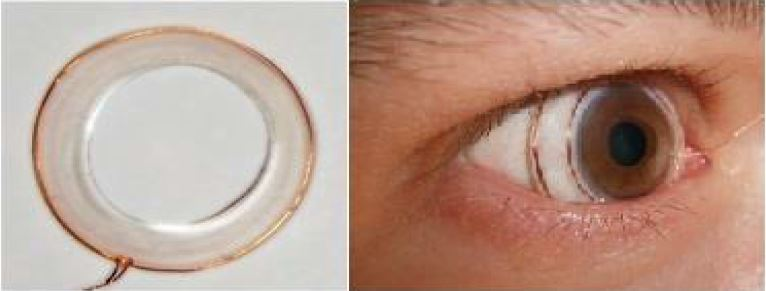
\includegraphics[width=0.7\linewidth]{figures/contact_lens}
		\caption{ردیابی چشم به وسیله لنز تماسی}
	\end{subfigure}
	\newline
	\begin{subfigure}{.8\textwidth}
		\centering
		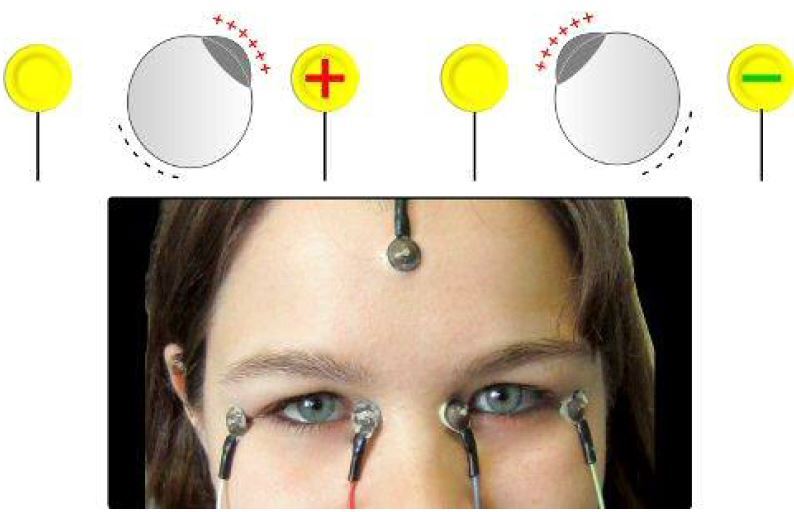
\includegraphics[width=0.7\linewidth]{figures/EOG}
		\caption{ردیابی چشم به وسیله بار الکتریکی}
	\end{subfigure}	
	\newline
	\begin{subfigure}{.8\textwidth}
		\centering
		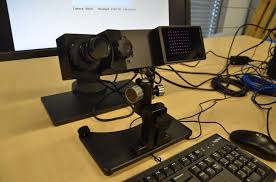
\includegraphics[width=0.7\linewidth]{figures/optical}
		\caption{ردیابی چشم با دوربین های نوری}
	\end{subfigure}

	\caption[ابزار های مختلف ردیابی چشم]{ابزار های مختلف ردیابی چشم}
	\label{fig:eyetech}
\end{figure}



\subsection{معیار‌های رهگیری چشم}
\label{ss:EyeMeasure}
اندازه‌گيری‌های فيزیولوژیک كه در دسته‌ی روشهای واقع‌گرایانه سنجش بار شناختی جای می‌گيرند،
ابزارهای مناسبی برای درک ارتباط بين حافظه‌ی كاری و یادگيری هستند. اغلب این اندازه‌گيری‌ها، امکان 
ثبت لحظه‌ای بار شناختی را فراهم می‌كنند .یکی از پركاربردترین این روشها، رهگيری چشمی است. 
داده‌هایی كه توسط دستگاه ردیاب چشم 
\LTRfootnote{Eye-tracker}
جمع‌آوری می‌شود در تحليل بسياری از فعاليت‌های شناختی
مورد استفاده قرار می‌گيرد.
\\
معيارهای مختلفی از داده‌های استخراج شده توسط دستگاه ردیاب چشم مورداستفاده قرار می‌گيرند،
برای مثال مدت زمان تثبيت چشم و نرخ پلک زدن در پژوهش‌های بسياری برای ارزیابی بار شناختی به كار 
رفته‌اند. برخی از این معيارها، ناشی از حركات ارادی چشم هستند و برخی غيرارادی اند. در ادامه، هر یک 
از این معيارها معرفی  خواهد  شد  و  ارتباط  هریک با  بار  شناختی بر  اساس  پژوهش‌های گذشته  بيان
می‌شود.
\\
حرکت چشم، شامل هر نوع حرکت ارادی و یا غیر ارادی برای پیدا کردن، تمرکز و دنبال کردن محرک های چشمی می‌گویند.

\subsubsection{تثبیت چشم}
رایج ترین رخدادی که در دستگاه رهیاب چشمی رخ می‌دهد، زمانی است که شخص در حالت تمرکز باشد و چشم ها در یک مدت زمانی ثابت باشند به این رویداد تثبیت چشم
\LTRfootnote{Fixations}
گویند. مدت آن از ۲۰۰ الی ۳۰۰ میلی‌ثانیه تا چند ثانیه خواهد بود و زاویه‌ای حدود 
$^\circ$۱
 است. این یک رویداد ارادی است. تعداد تثبیت ها نشان دهنده تعداد دفعاتی است که یک کابر به مکان خاص
\LTRfootnote{area of interest (AOI)}
نگاه کرده است.
پس حالت توجه با مکان خیره شدن در صحفه و یا مکان خاص مشخص می‌شود.
\\
رادمن و همکاران 
\cite{rudmann2003eyetracking}
متوجه شدند جهت خیره شدن نشان دهنده علت بار شناختی فعلی است. همچنین می‌توان از زمان تثبیت و یا خیرگی
\LTRfootnote{fixation duration}
به عنوان عامل نشان دهنده سطح بار شناختی استفاده نمود. این عمل با کاهش نرخ تثبیت همراه خواهد بود. چن و همکاران نشان دادند نرخ و زمان تثبیت با پیچیدگی آزمایش افزایش پیدا می‌کند.

\subsubsection{پرش چشم}

پرش چشم
\LTRfootnote{Saccades}
اشاره به حالتی دارد که که چشم بین دو موقعیت جابه‌جا می‌شود.
پرش چشم و خیرگی می‌توانند با استفاده از الگوریتم هایی که مکان طولی و عرضی مردمک را پردازش می‌کنند به صورت خودکار از یکدگیر جدا و برچسب گذاری‌ شوند.
به صورت ارادی است و پس از تثبیت رخ می‌دهد.
تثبیت و پرش چشم توسط سیگنالهای عصبی از سیستمهای قشر مغز و تحت قشر رمزگذاری می شود. این حرکت سریع ترین حرکتی است که بدن می‌تواند انجام دهد وبین ۳۰ تا ۸۰ میلی ثانیه طول می‌کشد تا انجام شود. رایج‌ترین شیوده تجسم پرش چشم، مسیرهای پویش
\LTRfootnote{Scanpath}
است. 
 می‌توان سرعت و طول پرش چشم‌ها را 
سنجيد و الگوهای مسير پویش را مشاهده كرد.
\cite{zagermann2016measuring}
چن و همکارانش، از اندازه‌گيری سرعت پرش چشم و 
طول آن به منظور بررسی تلاش ذهنی انسان استفاده كردند. نتایج آنها نشان داد كه سرعت و طول پرش 
چشم مولفه‌هایی  تفکيک  كننده  برای  دستیابی  به  كارآیی بالا  هستند.
\cite{chen2011eye}
همچنين،  مانوئل  و 
همکارانش دریافتند كه كاهش سرعت پرش چشم نشان دهنده خستگی و افزایش آن نمایان‌گر افزایش 
سختی كار است.
\cite{barrios2004adele}
بر اساس این یافته‌ها، بار شناختی با سرعت و طول پرش چشم نسبت مستقيم 
دارد؛ یعنی افزایش این دو شاخص، نشان دهنده افزایش بار شناختی است.
\paragraph{دامنه پرش}
یک ویژگی مفید دیگر، دامنه پرش
\LTRfootnote{Saccade Amplitude}
است، که اشاره به سختی دنبال کردن و یافتن دقیق مکان هدف مورد نظر دارد.
\cite{Hyona2003}
\subsubsection{گشادی قطر مردمک}
یکی دیگر از معيارهای چشمی گشاد شدن مردمک چشم
\LTRfootnote{Pupil dilation}
است،
عملکرد اصلی تغییر قطر مردمک محافظت از شبکیه (در برابر تابش نور) است و همچنین برای پاسخ به تغییر در تثبیت تصویر و واضح کردن آن برای اشیاء دور تا نزدیک.
تغییراتی که بازتاب تغییرات در فعالیتهای شناختی است در مقایسه با تغییرات ناشی از بازتاب نور و انعکاس اشیا نزدیک ، نسبتاً اندک است و علاوه بر آن تغییر در نور نسبتا سریع تر تغیرات مردمکی را در بر خواهد داشت.
بنابراین ، اگر اشیاء دارای عمق تقریباً ثابت در قسمت دیداری کاربر (بیمار) باشند، ما می‌توانیم داده های فرکانس پایین مردمک را استفاده کنیم.
\\
پس از دهه‌ها بررسی و مطالعه تغییرات مردمک هنوز محققان در منشا آن توافق ندارند، عده‌ای بر این باورند که منشا آن فشار ذهنی است و گروه دیگر برانگیختگی عاطفی را دلیل این تغییرات می‌دانند.
مشاهدات تجربی نشان می‌دهند مردمک در مواجه با تصاویر و صداهای بیشتر برانگیخته‌تر می‌شود، صرف نظر از بار احساسی ذاتی آن.
یک پژوهش اولیه روی بار احساسی و شناختی سعی بر ثابت نگه داشتن بارشناختی و ترکیب چند بار شناختی نمود نتیجه آن بود که بار شناختی تغییرات بیشتری در مردمک چشم ایجاد می‌کند.
\cite{Chen2013}
 پاسخ مردمک به عنوان یک واكنش غيرارادی رخ می‌دهد.
گشادی مردمک یک سیگنال فیزیولوژیکی است که که تغییراتش بسته به فعالیت های خودکار سیستم عصبی در دستگاه عصبی پیرامونی است.
قطر مردمک چشم می‌تواند بين  1/5 تا 8 ميلیمتر تغيير كند. روان‌شناسان در بيش از دو دهه اخير، تاكيد دارند 
تغييرات قطر مردمک، پردازش شناختی پرتلاشی را همراه دارد. پژوهش‌های گذشته نشان می‌دهند كه 
مردمک  بيننده  هنگامی  كه  سختی  كار  و  تلاش  شناختی  فرد  برای  پاسخ  به  آن  افزایش  می‌یابد،  گشاد 
می‌شود. مطالعه‌های زیادی اعتبار این استدلال را در كارهای مختلفی شامل مطالعه، حل مسئله و كارهای
دیداری تایيد كردهاند.
\cite{zagermann2016measuring}
همچنين پورتا و همکارانش، كاهش اندازه قطر مردمک در آستانه‌ی پایان كار در  آزمایش  خود  را  به  عنوان  نشانه‌ای  نهفته  برای  خستگی  قلمداد  كرده‌اند.
\cite{porta2012emotional}
علاوه  بر  فرآیندهای شناختی، تغييرات  در  روشنایی  محيط  تغييرات  در  اندازه  قطر  مردمک  را  در  پی  دارد.  با  تاریکتر  شدن محيط،  مردمک  چشم  برای  كسب  نور  بيشتر  گشاد  و  با  روشنایی  بيشتر  محيط، تنگ  می‌شود.  كنترل 
روشنایی محيط و درخشندگی نمایشگر یک چالش جدی در شرایط آزمایشگاهی است كه تغييرات در قطر مردمک  را  مطالعه  می‌كند.
\cite{zagermann2016measuring}
به  این ترتيب، افزایش  بار شناختی  باعث  گشادی مردمک چشم خواهد شد.
\subsubsection{پلک زدن}
چشم‌ما با هدف کاربری ۲ تا ۴ بار در دقیقه پلک می‌زند. اهداف غیر کاربردی دیگری مثل پلک‌زدن انعکاسی(یک پاسخ محافظ، مثل نزدیک شدن ناگهانی اشیا به سمت چشم)،‌ پلک‌زدن ارادی، پلک زدن درونی(غیر آگاهانه رخ‌ می‌دهد) و بسیاری از پلک‌زدن های ما از این نوع است که توسط سیستم عصبی مرکزی کنترل می‌شود و با شناخت ما ارتباط دارد. در نتیجه این نوع از پلک زدن ها برای اندازه گیری بار شناختی استفاده می‌شود.
\\
یک یافته نشان می‌دهد با افزایش تمرکز برای دریافت اطلاعات بیشتر از محرک نرخ پلک زدن کاهش می‌یابد دیدگاه دیگری در مقابل بیان می‌کند که پلک زدن مکانیزمی جهت آزادسازی و آسودگی است به طور مثال در هنگامی که به چیزی فکر نمی‌کنید و یا پایان آزمایش به ندرت پلک می‌زنید زیرا فشار ذهنی در هنگام حل مسئله بوده است. هنگامی که فشار ذهنی نتواند نمود درونی یا بیرونی پیدا کنید میزان پلک زدن افزایش می‌یابد.
باید سعی کنیم از طولانی بودن پنجره زمانی پلک زدن مطمئن شویم تا بتوان تغییرات محسوسی در هنگام اجرای آزمایش پیدا نمود.
\cite{Chen2013}

نرخ و تأخير در پلک زدن 
\LTRfootnote{Blink rate}
می‌تواند یک معيار رهگيری چشم دیگر در ارتباط با بار شناختی باشد.حرکت پلک‌ها توسط دستگاه عسبی مرکزی
\LTRfootnote{central nervous system (CNS)}
کنترل می‌شود.
 پلک زدن،  هرچند  می‌تواند  ارادی  هم  باشد،  یک  حركت  غيرارادی  در  نظر  گرفته  می‌شود.  نرخ  و  تأخير  پلک زدن‌ها، می‌تواند در فهم عميق درباره حالت توجه بيننده كمک كند.
\cite{zagermann2016measuring}
به عنوان مثال، تأخير زیاد و نرخ 
كم  پلک  زدن  به  عنوان  شاخصی  برای  تلاش  ذهنی  زیاد  دانسته  شده  است.
\cite{chen2011eye}
همچنين  مانوئل  و 
همکارانش، دریافتند كه افزایش نرخ پلک زدن و كاهش سرعت آن و نيز كاهش ميزان باز بودن پلکها، 
نشانه‌هایی برای افزایش خستگی هستند.
\cite{barrios2004adele}
بر اساس این یافته‌ها، می‌توان گفت: افزایش بارشناختی 
با كاهش نرخ پلک زدن و افزایش تأخير در پلک زدن نسبت مستقيم دارد. همچنين ممکن است بين بار 
شناختی و سرعت پلک زدن نيز رابطه‌ای وجود داشته باشد.
\subsubsection{ریزپرش چشم}
ریز پرش چشم
\LTRfootnote{Microsaccade}
یکی دیگر از حرکت‌های چشم است که توسط دستگاه ردیاب چشمی اندازه‌گیری می‌شود. ریزپرش‌‌ها غیر ارادی هستند همانند پرش‌ با دامنه کم هستند و در حالتی که چشم سعی در تثبیت دارد رخ می‌دهند.
\cite{Krejtz2018}
از جمله ویژگی‌های مثبت این معیار می‌توان به عدم حساسیت به میزان نور محیط اشاره کرد و دیگر آن‌ که با توجه به واکنش سریع و حساسیت این نوع حرکت می‌توان آن را در اندازه‌گیری بارشناختی به صورت همزمان استفاده نمود. 

\subsubsection{دنبال کردن روان}
دنبال کردن روان
\LTRfootnote{Smooth Pursuit}
اجازه می‌دهد چشم‌ها با فاصله نزدیکی یک شیء متحرک را دنبال کنند. به بیانی دیگر راهی برای تغییر مکان خیرگی است.
کاربر نمی‌تواند دنبال کردن روان را ارادی و به طور ساختگی انجام دهد چرا که نیاز است چشم‌ها به یک شیء متحرک قفل شوند و آن را دنبال کنند. نتایج آزمایش‌ها نشان داده با افزایش سختی آزمایش شیء با دقت و نظم کمتری دنبال می‌شود. در شکل 
\ref{fig:smoothpursuit}
می‌توانید نمونه نتیجه دنبال کردن روان را در دو حالت بار شناختی زیاد و کم مقایسه کنید.
\begin{figure}[htbp]
	\centering
	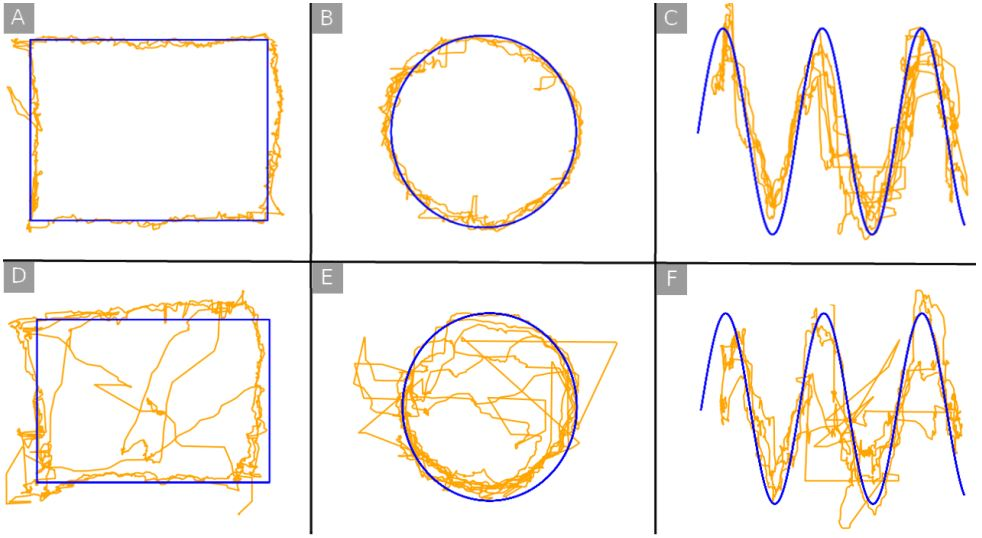
\includegraphics[width=0.7\linewidth]{figures/Smooth_Pursuit}
	\caption[آزمایش دنبال کردن روان یک شیء]{خطوط آبی مسیری است که شیء متحرک روی آن حرکت کرده و خطوط نارنجی مسیر دنبال کردن روان چشم است. ردیف بالایی حالتی است که کاربر بارشناختی کمی داشته و ردیف پایین بار شناختی بالا}
	\label{fig:smoothpursuit}
\end{figure}


\subsection{معیار‌های سیگنال مغزی}
ای‌ای‌جی یک روش محبوب تصویر برداری عصبی
\LTRfootnote{Neuroimaging}
است و با استفاده از الکترود‌های قرار گرفته بر روی سر به اندازه‌گیری فعالیت های الکتریکی مغز می‌پردازد. سنجش به کمک دستگاه ای‌ای‌جی به دلیل ثبت لحظه‌ای و پیوسته سیگنال‌های مغزی و می‌تواند به خوبی نشان دهنده کوچکترین تغییرات در بارشناختی بر اثر انجام آزمایش‌های مختلف باشد، از این رو استفاده از آن بسیار امیدوار کننده است . در ادامه فرایند‌های ثبت و تحلیل و سپس معیار‌های استخراج شده از آن برای سنجش بار شناختی بررسی می‌شود.
\subsubsection{باندهای مختلف سیگنال مغزی}
با توجه به فرکانس‌های امواج مغز آن‌ها را به پنج دسته یا باند تقسیم کرده‌اند. در شکل
\ref{fig:this-frequency-bands-of-eeg-signal}
می‌توانید نمونه این پنج دسته را مشاهده کنید. از این میان دو باند به دشواری فعالیت گزارش شده‌اند، آلفا و تتا. معمولا چگالی طیف توان
\LTRfootnote{Power Spectral Density}
 هر باند محاسبه می‌شود و سپس از آن برای مطالعه آزمایش مورد نظر استفاده می‌شود.
 \\
 مغز انسان در حالات مختلف مانند بیداری، خواب و یا خشم فرکانس‌های متفاوتی از خود بروز می‌دهد همچنین ویژگی‌های این امواج با تغییر سن نیز تغییر می‌کنند. 
 در ادامه به صورت جداگانه به بررسی هریک از باند‌های مغز می‌پردازیم.
\begin{figure}[htbp]
	\centering
	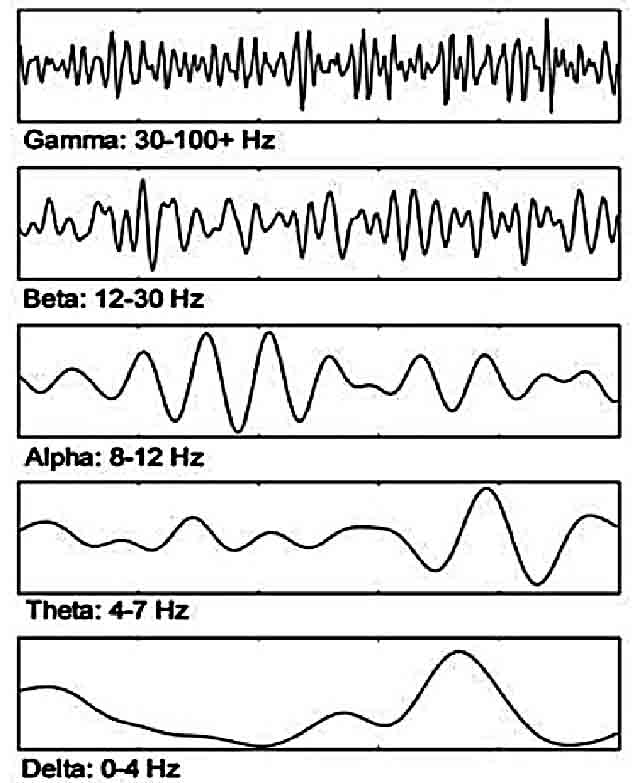
\includegraphics[width=0.5\linewidth]{figures/This-Frequency-bands-of-EEG-signal}
	\caption[باندهای امواج مغزی]{پنج باند فرکانس مغزی از بیشترین فرکانس در ردیف اول تا کمترین فرکانس در ردیف آخر نمایش داده شده‌است}
	\label{fig:this-frequency-bands-of-eeg-signal}
\end{figure}

\subsubsection*{امواج گاما - $ \gamma $}
فرکانس ریتم یا امواج گاما در محدوده بین ۳۰ تا ۱۰۰ هرتز قرار دارد. این امواج با ورودی‌های حسی و همچنین حافظه و توجه مرتبط هستند.
در برخی از تحقیقات، فعالیت‌های غیرمعمول در امواج گاما، برای بیماری‌هایی چون پارکینسون و صرع و آلزایمر گزارش شده‌است. همچنین در اختلال‌های خُلقی مثل افسردگی عمده و اختلال دوقطبی نیز دیده شده است.
\subsubsection*{امواج بتا - $ \beta $}
این امواج در فرکانس بین ۱۲ تا ۳۰ هرتز قرار دارند. باند بتا نمایانگر حالتی در مغز هستند که در هوشیاری معمول اتفاق می‌افتند. در فعالیت‌هایی مانند تفکر و یا توجه فعال، تمرکز، حل مسئله در بزرگسالان نرمال وجود دارد. این امواج در نواحی جلویی و مرکزی مغز وجود دارند، سطح بالای آن می‌تواند نشان دهنده وحشت باشد.
\subsubsection*{امواج آلفا - $ \alpha $}
معمولا فرکانس این امواج در ناحیه ۸ تا ۱۲ هرتز قرار دارد. این امواج معمولا با بسته شدن چشم‌ها در حالت استراحت، آرامش و خواب سبک ظاهر می‌شوند و در حالت خواب عمیق و یا اضطراب از بین می‌روند. میان افراد خلاق و سایرین در این ریتم تفاوت دیده شده است؛ به نحوی که در هنگام حل یک مسئله جدید هستند و ایده جدیدی دارند در نیمکره چپ مغز خود امواج آلفای بیشتری نسبت به بقیه تولید می‌کنند. این امواج معمولا در قسمت آکسیپیتال ظاهر می‌شوند.
\subsubsection*{امواج تتا - $ \theta $}
عموما این امواج در فرکانس ۴ تا ۷ هرتز قرار دارند. این امواج معمولا در هنگامی که هوشیاری به سمت خواب‌آلودگی می‌رود ظاهر می‌شوند. این امواج به سادگی در قسمت هیپوکمپوس
\LTRfootnote{hippocampus}
مشاهده می‌شوند البته ممکن است در سایر نواحی با احساسات مختلف نیز ظاهر شوند. در آزمایش‌هایی که حافظه کوتاه مدت را مورد بررسی قرار می‌دهند نیز دیده شده است.
\cite{vertes2005hippocampal}

\subsubsection*{امواج دلتا- $ \delta $}
 امواج دلتا در محدوده بیشتر از صفر  تا ۴ هرتز قرار می‌گیرند. این ریتم را به حالت خواب عمیق و آرام نسبت داده‌اند. ممکن است با نویز امواجی که از حرکت عضلات فک و گردن تولید می‌شوند اشتباه گرفته شود که البته به کمک نرم‌افزار‌های پردازش داده‌های مغزی میتوان آن‌ها را از یکدیگر تمیز داد. در بیماری‌های چون اسکیزوفرنی و پارکینسون نیز ظهور این امواج دیده شده است.
\subsubsection{استفاده از تغییرات، بجای قدرت سیگنال}
در پژوهش‌هایی که از داده‌های ‌ای‌ای‌جی استفاده می‌کنند معمولا از تغییرات سیگنال حاصل شده از یک کار یا فعالیت خاص بجای قدر مطلق قدرت
\LTRfootnote{Absolute power}
آن سیگنال استفاده می‌کنند. دلیل این امر آن است که مشاهدات نشان داده اند رفتار امواج مغزی با توجه به تفاوت‌های فردی، حجم مغز و سن افراد تفاوت پیدا می‌کند. از این رو از معیار
\lr{event related de-synchronization}
یا به اختصار
\lr{ERD/ERS}
استفاده می‌کنند.
معمولا در آزمایش و فعالیت های پژوهشی که داده مغزی گرفته می‌شود حاتی را نیز در نظر می‌گیرند که از او هیچ کاری نمیخواهند و فعالیتی انجام نمی‌دهد به این حالت باز پایه یا مرجع
\LTRfootnote{Baseline}
 می‌گویند.
 \\
 ERD/ERS
 طبق رابطه 
 \ref{eq:ERD-ERS}
 تعریف می‌شود.
 \begin{equation}\label{eq:ERD-ERS}
 \text{ERD/ERS}\% = \dfrac{\text{baseline interval band power - test interval band power}}{\text{baseline interval band power}}\times 100
 \end{equation}
 رابطه 
 \ref{eq:ERD-ERS}
را می‌توان اینگونه توضیح داد که 
ERD/ERS
نشان دهنده درصد افزایش یا کاهش قدرت باند در طول بازه مد نظر نسبت به بازه‌ی پایه.
این شاخص برای دو باند آلفا و تتا در بسیاری از آزمایش‌های شناختی حساس نسبت به سطح دشواری کار است.
\subsection{مزایا و معایب استفاده از سیگنال‌های مغزی}
\label{bbc:eeg_procon}
\paragraph{نقاط قوت}
اکثر روش‌های ثبت و سنجش فعالیت های مغزی یا نیازمند تجهیزات گران قیمت و پیشرفته که جهت کار با آنها نیاز به دانش پزشکی هستند و یا کار با آن‌ها برای آزمایش‌دهنده آسان نیست. همانند برش‌نگاری با گسیل پوزیترون
\LTRfootnote{Positron Emission Tomography - PET scan}
که نیازمند خوردن مواد خطرناک توسط آزمایش دهنده هستند یا دستگاه fMRI که فرد باید در حالت دراز کشیده بدون حرکت باشد، با این حال دستگاه‌های ثبت سیگنال مغزی بسیار کوچک‌‌تر و حتی نسخه‌های قابل حمل آن نیز موجود می‌باشد و تنها نیازمند به شرایط  معمول آزمایش‌گاهی است.
\\
ثبت سیگنال مغزی به وسیله ای‌ای‌جی از دقت زمانی بسیار خوبی (میلی‌ثانیه) بهره می‌برد از این رو میتوان به صورت پیوسته کوچک‌ترین مداخلات شناختی را شناسایی و اندازه‌گیری کرد.
\\
نرم‌افزار های قدرتمندی که در کنار این دستگاه‌ها استفاده می‌شوند توانایی خوبی در حذف و فیلتر کردن اثرات ناخواسته و یا نویز‌ها را دارند.
\paragraph{نقاط ضعف}
داده‌های
EEG
از دقت مکانی کمی برخوردار هستند (حدود سانتی متر) از این رو نمی‌توان به طور دقیق مکان فعالیت‌های مغزی را ثبت نمود. یکی دیگر از ضعف‌های داده‌های 
EEG
 نویز پذیر بودن آن است، این سیگنال‌ها می‌توانند به راحتی توسط حرکاتی چون: پلک زدن، نفس کشیدن، ضربان قلب، فرو بردن آب دهان و یا تکان خوردن سر تحت تاثیر قرار بگیرند که گاها این سیگنال‌ها از فعالیت‌های عصبی قوی‌تر هستند.
 \cite{antonenko2010using}
\subsection{ثبت سیگنال مغزی}
همان گونه که در شکل
\ref{fig:fnhum-05-00089-g002}
مشاهده می‌کنید اجزا تشکیل دهنده دستگاه ثبت سیگنال مغزی از سه قسمت تقویت کننده، ذخیره کننده و نمایش دهند سیگنال ها تشکیل شده است.
\begin{figure}[htbp]
	\centering
	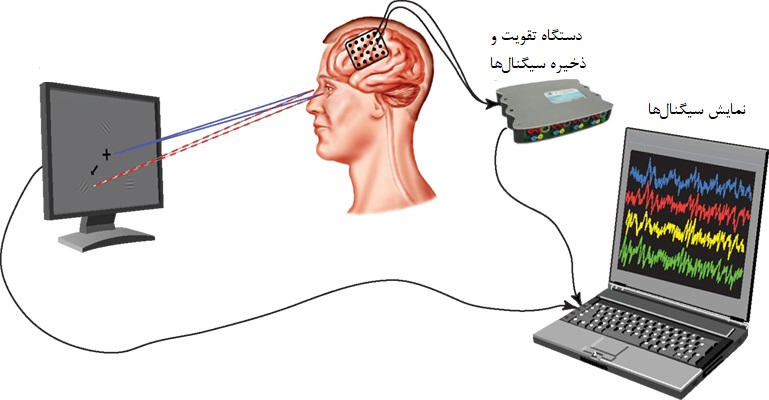
\includegraphics[width=0.9\linewidth]{figures/fnhum-05-00089-g002}
	\caption[اجزا دستگاه ثبت سیگنال مغزی]{حسگر‌ها داده‌های فعالیت های الکتریکی مغز را به تقویت کننده و ذخیره کننده سیگنال‌ها می‌فرستند و سپس توسط سیستم به نمایش در می‌آیند.}
	\label{fig:fnhum-05-00089-g002}
\end{figure}
\\
وجود بافت‌های ضخیمی مثل، استخوان، ماهیچه و خون در مسیر عبور سیگنال‌های مغزی  از محل تولید آن در قشر مغز تا محل قرارگیری الکترود‌های گیرنده، اندازه این سیگنال‌ها به شدت ضعیف می‌شوند از این رو جهت قابل مشاهده و استفاده بودن آن‌ها از تقویت کننده‌هایی برای تقویت آن‌ها استفاده می‌شود.
\cite{kheradpisheh2014evidence}
جهت ثبت با کیفیت بهتر سیگنال‌های مغزی میزان اتصال آن‌ها با پوست سر اهمیت دارد از این رو از ژل های مخصوصی جهت رسانایی بیشتر استفاده می‌شود.
\\
به جهت امکان مقایسه نتایج داده‌های EEG پژوهشگران، استانداردی تحت عنوان ۱۰-۲۰ که مکان الکترودها را روی قشر‌های مختلف مغز مشخص می‌کند ایجاد شده است. عددهای ۱۰ و ۲۰ در نام این روش، بیانگر این موضوع هستند که فاصله بین دو الکترود متوالی، همواره برابر با ۱۰٪ یا ۲۰٪ اندازه فاصله جلو-عقب سر یا فاصله راست تا چپ سر است. در این حالت تعداد الکترود‌های به کار رفته ۲۱ عدد است در برخی کاربرد‌ها تعداد بیشتر الکترود نیز ممکن است.
\\
در این روش مکان هر الکترود با دو کاراکتر مشخص می‌شود.

کاراکتر نخست، که یک حرف انگلیسی است، بیانگر قسمتی از نواحی مغز است که الکترود روی آن قرار می‌گیرد و کاراکتر بعدی که یک عدد است، بیانگر نیم کره راست و چپ مغز است. در جدول
\ref{tab:EEG_CHAR}
نمادها و معنای آن‌ها را می‌بینید.
\begin{center}
	\begin{table}[h]
	\centering
	\caption{نمادهای استفاده شده در استاندارد ۱۰-۲۰ التروانسفالوگرافی}
	\label{tab:EEG_CHAR}
	\begin{tabular}{|c|c|c|c|c|c|c|c|c|}
		\hline
		اعداد فرد    & اعداد زوج  & z      & O      & P         & C     & T        & F      &\textbf{ نماد}      \\ \hline
		نیم کره راست & نیم کره چپ & فرق سر & پس‌سری & آهیانه‌ای & مرکزی & گیج‌گاهی & پیشانی & \textbf{ناحیه مغز} \\ \hline
	\end{tabular}
\end{table}
\end{center}
در شکل
\ref{fig:LOB_1020}
محل قرارگیری الکترودها و لو‌ب‌های مغز را می‌بینید.
به جهت پرهیز از اندازه‌گیری های وقت‌گیر و دقت بیشتر در اندازه‌گیری سیگنال‌های مغزی الکترود ها را مطابق استاندارد ۱۰-۲۰ می‌توان بر روی یک کلاه  قرار داد، در این صورت با قرار دادن کلاه بر روی سر خودبه‌خود الکترود ها در مکان مناسب قرار می‌گیرند. نمونه‌ای از آن را در شکل 
\ref{fig:eegcap}
می‌بینید.
\begin{figure}[htbp]
	\centering
	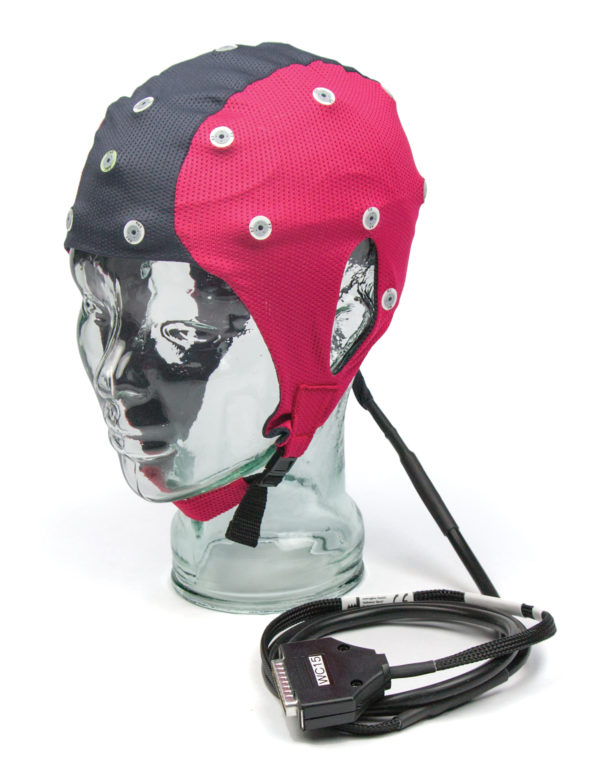
\includegraphics[width=0.3\linewidth]{figures/EEG_cap}
	\caption[کلاه ثبت سیگنال مغزی]{استفاده از کلاه ثبت سیگنال مغزی به منظور اندازه‌گیری دقیق و ساده‌تر}
	\label{fig:eegcap}
\end{figure}

\begin{figure}[htbp]
	\centering
	\begin{subfigure}{\textwidth}
		\centering
		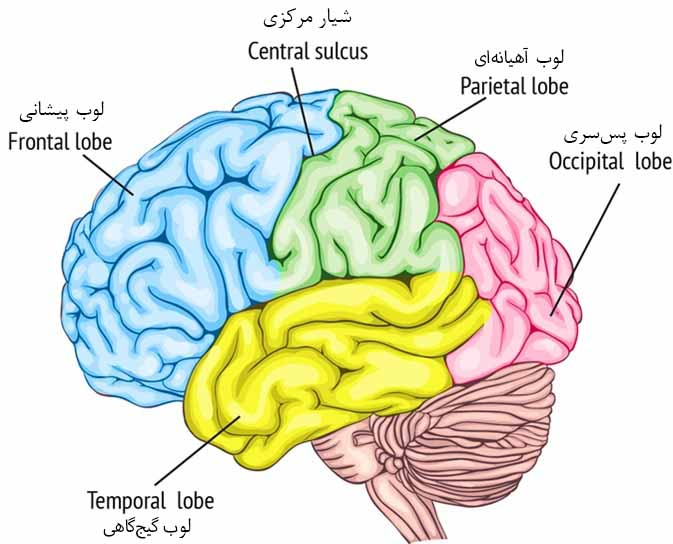
\includegraphics[width=.7\linewidth]{figures/brain_lobes}
		\caption{طرحی از مغز و چهار لوب آن}
		\label{fig:brainlobes}
	\end{subfigure}
	\begin{subfigure}{\textwidth}
		\centering
		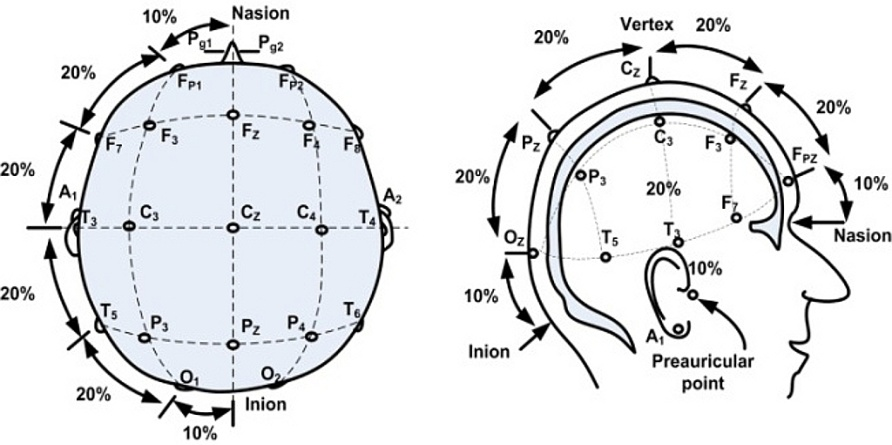
\includegraphics[width=\linewidth]{figures/EEG_10-20}
		\caption{نقاط قرارگیری الکترود‌های دستگاه الکتروانسافلوگراف بر روی سر مطابق استاندارد ۱۰-۲۰}
		\label{fig:eeg10-20}
	\end{subfigure}
	\caption[لوب‌های مغز و استاندارد ۱۰-۲۰]{مکان قرارگیری الکتوردهای دستگاه الکتروانسافلوگراف و لوب‌های مغز}
	\label{fig:LOB_1020}
\end{figure}


% 5- Data process and Litreture review
\section{پردازش و موارد مطالعه داده‌های ‌چشمی و مغزی در اندازه گیری بارشناختی}
\label{s:data}
\subsection{صاف کردن و حذف نویز از داده‌های سیگنال مغزی}
در بخش
\ref{bbc:eeg_procon}
نویزهای مختلفی که می‌ تواند بر سیگنال دریافتی اثر بگذارد را دیدیم، گاهی این نویزها به قدری شبیه به امواج مغزی هستند که حتی افراد متخصص و با تجربه نیز نمی‌توانند به سادگی آن‌ها را از سیگنال اصلی تشخیص دهند. نویزها را می‌توان با توجه به عامل تولید کننده آن به دو دسته فیزیولوژیکی و غیر فیزیولوژیکی تقسیم کنیم. از جمله نویزهای فیزیولوژیکی که منشأ آن حرکات بدن است می‌توان به پلک زدن، حرکت سر، حرف زدن، بلعیدن و فعالیت الکتریکی قلب اشارده نمود، در دسته دیگر توزیع برق شهری، جابه‌جایی التکرودها بر روی سر و نویز تجهیزات ثبت سیگنال مثال‌هایی از غیر فیزیولوژیک هستند.
در شکل 
\ref{fig:eeg-blink-noise}
نمونه‌ای از نویز پلک زدن را مشاهده می‌کنید.
\begin{figure}[h]
	\centering
	\includegraphics[width=0.7\linewidth]{"figures/EEG blink noise"}
	\caption[نویز پلک زدن]{در قسمت‌های هاشور زده نمونه نویز پلک‌زدن مشخص شده‌است}
	\label{fig:eeg-blink-noise}
\end{figure}
جهت حذف نویز می‌توان ابتدا به صورت دستی فرکانس‌های بسیار بالا و پایین را حذف نمود و سپس از ابزار‌های آماده استفاده نمود. در فضای فرکانس با فیلتر بالا گذر
\LTRfootnote{High Pass Filter}
با فرکانس قطع ۰.۵ هرتز مي‌توان فرکانس نفس کشیدن را حذف نمود و برای اطمینان از حذف نویز برق شهری فرکانس ۵۰ هرتز با ناچ فیلتر
\LTRfootnote{Notch Filter}
حذف می‌شوند. از آن‌جا که الگوهای نویزهای یک دسته شبیه به هم هستند ابزار های هوشمندی چون جعبه ابزار کار با ای‌ای‌جی متلب به صورت خودکار آن‌ها را شناسایی کرده و حذف می‌کند.
\subsection{روش‌‌های استخراج ویژگی از داده‌های سیگنال مغزی}
ویژگی را می‌توان یک خصوصیت متمایز، اندازه‌گیری قابل تشخیص و یک مولفه کاربردی دانست که از بخشی از یک الگو بدست بیاید. به استخراج بخش‌های مهم اطلاعات و حذف  سایر قسمت‌های آن استخراج ویژگی  می‌گویند. برای به حداقل رساندن از بین رفتن اطلاعات مهم تعبیه شده در سیگنال، از استخراج ویژگی استفاده می‌شود. علاوه بر این، ویژگی‌ها میزان منابع مورد نیاز برای توصیف دقیق مجموعه عظیمی از داده ها را ساده‌تر می کنند. ویژگی‌ها برای به حداقل رساندن پیچیدگی های پیاده سازی برای کاهش هزینه پردازش اطلاعات و به منظور رفع نیاز احتمالی برای فشرده سازی اطلاعات استفاده می‌شوند.
\cite{al2014methods}
\\
اخیراً روش‌های متنوعی برای استخراج ویژگی‌ها از سیگنال‌های EEG به‌کار گرفته شده است، از میان آن‌ها می‌توان به این تبدیل‌ها اشاره نمود:
\begin{itemize}
	\item توزیع فرکانس زمان
	\LTRfootnote{time frequency distributions - TFD}
	\item تبدیل فوریه سریع
	\LTRfootnote{fast fourier transform - FFT}
	\item روش‌های مبتنی بر بردار ویژه
	\LTRfootnote{eigenvector methods - EM}
	\item تبدیل موجک گسسته
	\LTRfootnote{discrete wavelet transform - DWT }
	\item روش‌ خود همبسته
	\LTRfootnote{auto regressive method - ARM}
\end{itemize}
به جهت استفاده بیشتر از دو روش تبدیل فوریه سریع و تبدیل موجک گسسته در ادامه شرح این دو روش را خواهیم دید.
\subsubsection{تبدیل فوریه سریع}
\label{sssection:FFT}
سیگنال‌های EEG از شلیک یا اسپایک
\LTRfootnote{Spike}
همزمان نورون‌های عصبی شکل می‌گیرد و در طبیعت از فعالیت های دنبال شونده در طیف گسترده ای از فرکانس تشکیل شده است از این رو معمولا سیگنال‌های EEG را در فضای فرکانس تحلیل می‌کنند.
\cite{hu2019eeg}
در تبدیل فوریه، سیگنال مغزی که در حوزه زمان است را به حوزه فرکانس می‌بریم. این تبدیل مؤلفه‌های فرکانس ‌های موهومی یک سیگنال در حالت کلی نامتناوب را استخراج و نمایان می‌کند، در واقع تبدیل فوریه یک سیگنال، وزن فرکانس‌های موهومی موجود در سیگنال را نشان می‌دهد. به تبدیل فوریه یک سیگنال، طیف سیگنال
\LTRfootnote{Signal Spectrum}
 نیز گفته می‌شود.
 رابطه 
 \eqref{eq:DTFT}
 تبدیل فوریه سیگنال زمان گسسته
$  x_{n} $
 را نشان می‌دهد.
 \begin{equation}\label{eq:DTFT}
 X_{K}=\sum_{n=0}^{N-1}x_{n}e^{-i2\pi kn/N}
 \end{equation}
 که در آن N تعداد نمونه‌ها و n نمونه‌ فعلی است. $ x_{n} $ نشان دهنده مقدار سیگنال در زمان n و k  فرکانس فعلی (۰ هرتز تا N-1 هرتز) و $ X_{k} $ نتیجه حاصل از تبدیل فوریه گسسته است.
 محاسبه مستقیم تبدیل فوریه از رابطه
 \eqref{eq:DTFT}
 کند بوده و زمان زیادی می‌برد از این رو از الگوریتم تبدیل فوریه سریع که به صورت بازگشتی و با تقسیم و غلبه کار‌ می‌کند استفاده می‌کنند.
 شکل 
 \ref{fig:signal-analysis}
 به درک بهتر این تبدیل کمک می‌کند.
 \begin{figure}[h]
 	\centering
 	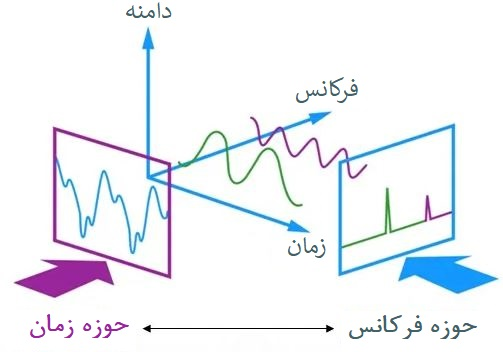
\includegraphics[width=0.7\linewidth]{figures/Signal-Analysis}
 	\caption[تبدیل فوریه]{تبدیل فوریه یک سیگنال دلخواه را از فضای زمان و یا مکان به فضای فرکانس می‌برد.\cite{fourier_transform}
 	}
 	\label{fig:signal-analysis}
 \end{figure}
 ولچ
 \LTRfootnote{Welch}
 یک روش بدون پارامتر تخمین همبستگی خودکار
 \LTRfootnote{autocorrelation}
 است. سیگنال‌های ثبت شده توسط تخمین چگالی توان (PSD)
 \LTRfootnote{power spectral density - PSD}
 محاسبه‌‌ می‌شوند. تا به صورت انتخابی نمایانگر نمونه‌های ای‌ای‌جی باشند.
\subsubsection{تبدیل موجک گسسته}
\label{sssection:DWT}
تبدیل فوریه تا زمانی که فرکانس‌های ظاهر شده در یک سیگنال وابسته به زمان نباشند به خوبی عمل خواهد کرد یا به عبارت دیگر اگر یک سیگنال شامل فرکانس x هرتز باشد، این فرکانس باید به صورت برابر در تمام طول سیگنال وجود داشته باشد.
دسته‌ی زیادی از سیگنال‌ها در طبیعت که فرکانس‌ ‌آن‌ها در طول زمان تغییر می‌کند را نا نمی‌توان با تبدیل فوریه با دقت و رزولوشن خوبی مدل کرد. از جمله این سیستم‌های دینامیک میتوان به داده‌های بازار بورس، بدن انسان و داده‌های برخی تجهیزات اشاره کرد. در این شرایط از تبدیل موجک که هم اطلاعات فرکانسی و هم اطلاعات زمانی را ذخیره می‌کند استفاده می‌کنیم.
\\
بنابراین در حالت کلی می‌توان گفت تبدیل موجک به صورت توافقی عمل می‌کند. در مقیاس‌هایی که مشخصه‌های وابسته به زمان مهم‌تر هستند، تبدیل موجک دارای دقت بالاتر در حوزه زمان و در مقیاس‌هایی که مشخصه‌های وابسته به فرکانس مهم‌تر هستند، دارای دقت بالاتر در حوزه فرکانس است. این نوع توافق دقیقا همان هدفی است که در پردازش سیگنال مورد نظر است.
\\
تبدیل موجک سیگنال یک بعدی ای‌ای‌جی، دارای دو بعد است. این خروجی دو بعدی مربوط به تبدیل موجک، نمایش سیگنال اصلی بر حسب مقیاس و زمان است که به طیف اسپکتروگرام 
\LTRfootnote{Spectrogram}
 یا اسکالوگرام
\LTRfootnote{Scaleogram}
معروف است. تبدیل موجک انواع متفاوتی دارد. برای انواع مختلف تبدیل موجک، مصالحه بین فشردگی 
\LTRfootnote{Compact}
 و صاف بودن 
\LTRfootnote{Smooth}
  با یکدیگر تفاوت دارند. به عبارت دیگر این خاصیت بیان می‌کند که می‌توانیم نوع خاصی از تبدیل موجک را انتخاب کنیم که با ویژگی مورد نظر برای استخراج از سیگنال تناسب بیشتری داشته باشد. یکی از انواع معرف آن هار
  \LTRfootnote{Haar}
  است.
  \\
روند کار در تبدیل موجک را در شکل 
  \ref{fig:wavelet-transform}
مشاهده می‌کنید.
در سطح صفرم ما یک سیگنال داریم و آن‌را در سطح اول به دو بخش تقریب
\LTRfootnote{Approximation}
 و جزئیات
\LTRfootnote{Detail}
  سیگنال تقسیم می‌کنیم. معمولا انتظار داریم نویز در بخش جزئیات باشد چون معمولا فرکانس نویز بالا است، تقریب اول شباهتش به سیگنال اصلی بیشتر است، از این رو می‌توان همان گونه که سیگنال اصلی را به دو بخش تجزیه کردیم تقریب اول را هم به دو بخش تقریب سطح دوم و جزئیات سطح دوم تجزیه می‌کنیم. این روند را تا جایی که جزئیات صفر و یا نزدیک به صفر شود انجام می‌دهیم . حال می‌توان سیگنال اصلی را با رابطه
  \eqref{eq:WaveletTransfrom}
  نشان داد. معمولا اگر به خواهیم نویزی را حذف کنیم از $ d_1 $ حذف می‌کنیم.
  
  \begin{equation}\label{eq:WaveletTransfrom}
  S = d_1 + d_2 + \cdots + d_N + a_N   
  \end{equation}
  اکنون به جای آنکه مستقیما سیگنال اصلی را به الگوریتم خود که می‌تواند شبکه عصبی، سیستم فازی یا شبکه بیزی
  \LTRfootnote{Bayesian network}
   باشد بدهیم، می‌تواینم ویژگی‌های استخراج شده یعنی $ d_1 $ تا $ d_N $ را بدهیم.
  \begin{figure}[h]
	\centering
	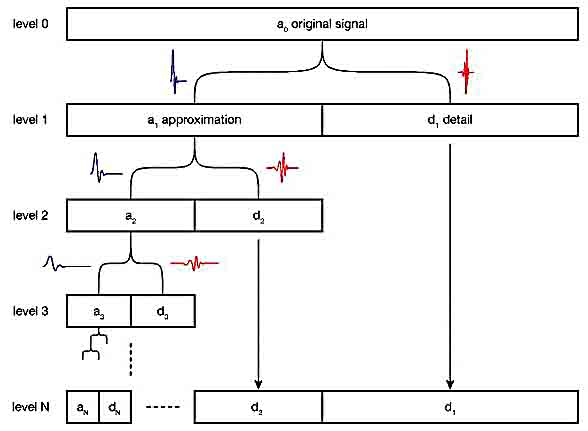
\includegraphics[width=\linewidth]{figures/wavelet-transform}
	\caption[تبدیل موجک]{بررسی اجمالی طرح تبدیل موجک گسسته، سیگنال اصلی به اجزای فرکانس پایین و فرکانس بالا تقسیم می شود ، که به ترتیب تقریب سیگنال و اطلاعات جزئیات را تشکیل می دهند. هر سطح اطلاعات تقریبی را بیشتر تجزیه می کند ، و هر سطح جزئیات یک باند فرکانس جداگانه را تشکیل می دهد\cite{sundling2006wavelets}}
	\label{fig:wavelet-transform}
\end{figure}

\subsubsection{مقایسه روش‌های استخراج ویژگی}
در دو زیر بخش
\ref{sssection:FFT}
و
\ref{sssection:DWT}
به ترتیب با تبدیل فوریه سریع و تبدیل موجک آشنا شدیم در این قسمت قصد داریم تا این دو تبدیل را با هم مقایسه و مزایا و معایب هریک را عنوان نماییم. استفاده مناسب از هر کدام می‌تواند راه حل خوبی باشد.
\\
در جدول
\ref{tab:FFT-VS-DWT}
می‌توانید مقایشه این دو روش را مشاده نمایید.

\begin{table}[]
	\caption[مقایسه تبدیل فوریه و موجک]{مقایسه مزایا و معایب دو روش تبدیل فوریه سریع و تبدیل موجک گسسته}
	\label{tab:FFT-VS-DWT}
	\begin{tabular}{ccc}
		\hline
		نام روش                                                        & مزیت‌ها                                                                                                                                                                                                 & معایب                                                                                                                                                                 \\ \hline
		\begin{tabular}[c]{@{}c@{}}تبدیل\\  فوریه\\  سریع\end{tabular} & \begin{tabular}[c]{@{}c@{}}-اغلب می‌تواند برای سیگنال‌های ایستا\\ (میانگین و واریانس در طول زمان ثابت باشد)\\  خوب عمل کند\\ -برای کارهای بلادرنگ \\ \\ تقریبا سریع تر از روش‌های دیگر است\end{tabular} & \begin{tabular}[c]{@{}c@{}}برای سیگنال‌هایی که فرکانس آن\\  در طول زمان تغییر کند مناسب نیست-\\ نمی‌تواند پیک‌های موجود را\\  با رزلوشن مناسبی  نشان دهد\end{tabular} \\ \hline
		\begin{tabular}[c]{@{}c@{}}تبدیل\\  موجک\end{tabular}          & \begin{tabular}[c]{@{}c@{}}اندازه پنجره آن متغییر است-\\ بین زمان و فرکانس مصالحه دارد-\\ -برای تجزیه و تحلیل سیگنال‌های\\  دارای تغییرات ناگهانی مناسب است\end{tabular}                                & -نیازمند انتخاب موجک مدار مناسب                                                                                                                                       \\ \hline
	\end{tabular}
\end{table}
\subsection{موارد مطالعه‌ی استفاده از داده‌های مغزی در سنجش بارشناختی}
در این زیر بخش به تعدادی پژوهش برجسته که در آن‌ها رابطه میان بارشناختی و سیگنال مغزی بررسی شده است خواهیم پرداخت. از میان آن‌ها نیز پژوهش‌هایی که به طور خاص با آزمایش‌ها و فعالیت‌هایی که محرک آن‌ها چند رسانه‌ای است در این مرور نقش مهم‌تری دارند.
\\
جِروْ و همکاران
\cite{gerve1999multimedia}
به بررسی بارشناختی حاصل یادگیری از چندرسانه‌ای از طریق سیگنال‌های مغزی پرداختند. در آزمایش آن‌ها که ۳۸ دانش آموزش مشارکت داشتند ۱۹ نفر مستعد و ۱۹ نفر معمولی. سه دسته محرک نمایش داده شد. متن؛ متن، تصویر و صدا؛ متن،‌صدا و فیلم و  در این حال امواج مغزی آن‌ها ثبت می‌شد. در طول نشان دادن متن مشاهده شد که توان باند آلفا بیشترین دامنه (فعالیت ذهنی کمتر) را در لوب‌های پس‌سری و گیج‌گاهی دارد و دامنه کم آن (فعالیت ذهنی بالاتر) در لوب پیشانی دیده شد. همچنین آن‌ها دیدند که دانش‌آموزان مستعد در هر سه محرک فعالیت ذهنی کمتری دارند.
\\
یزدانی و همکاران 
\cite{yazdani2009implicit}
به معرفی یک واسط رایانه مغز پرداختند که می‌تواند به صورت ضمنی محتوای‌ چندرسانه‌ای را از لحاظ احساسات مختلف برچسب بزند؛ به طوری که حتی داده‌های فردی که هنوز در آزمایش شرکت نکرده بود نیز به خوبی  قابل پیش‌بینی بود. در آزمایش آن‌ها نیز ۹ دانشجوی دکتری شرکت کرده بودند و از آن‌ها داده های سیگنال مغزی در حالی که چندرسانه‌ای را نگاه می‌کردند گرفته می‌شد.
\\
کاسترو و همکاران
\cite{castro2020validating}
به اعتبارسنجی باند تِتا به عنوان یک معیار عینی برای اندازه‌گیری بارشناختی در فیلم‌های آموزشی پرداختند. آن‌ها سه متن با سختی‌های متفاوت تولید کردند که یک راوی آن‌ها را می‌خواند. از شرکت کنندگان علاوه بر داده‌های مغزی و پرسشنامه فعلایت ذهنی، آزمون یادآوری نیز گرفته می‌شد. آن‌ها مشاهده کردند باند تتا و آزمون یادآوری برای ساده‌ترین و سخت ترین به خوبی می‌توانند تمیز دهنده این دو وضعیت باشند.
\\
آن‌ها فیلم‌های سخنرانی خود را به کمک دو معیار سطح بندی کردند. معیار اول سهولت خواندن
\LTRfootnote{reading ease}
بود. این معیار خوانایی متن را با شمارش تعداد هجا‌ها، کلمات و جملات انجام می‌دهد. خروجی آن یک عدد بین صفر تا صد است که هرچه بیشتر باشد نشان دهنده ساده‌تر و خوانایی بیشتر متن است. معیار دوم سهولت نحوی
\LTRfootnote{Syntactic simplicity}
بود. این معیار بر اساس چگالی عبارات اسمی، گروه معنایی کلمه‌ها و کلاس یک کلمه یک خروجی عددی می‌دهد که هرچه این عدد بزرگتر باشد نشان دهنده ساده‌تر بودن آن است. در آزمایش آن‌ها نیز ۳۵ نفر شرکت کرده بودند.
\\
آنتنکو و نایدرهاوسر
\cite{antonenko2010influence}
به بررسی بارشناختی حاصل از مطالعه متون حاوی هدایت‌گر از طریق سیگنال مغزی پرداختند. تفاوت میان متن معمولی و متن دارای هدایت‌گر در این است که در متن معمولی اگر خواننده به مفهومی برخورد کند که معنای آن را نداند باید از حافظه بلند مدت خود آن را به حافظ فعال فراخوانی و یادآوری کند از طرفی دیگر ساختمان و چینش مفاهیم دست نویسنده متن است. این در حالی است که در متن شامل هدایت‌گر خواننده هرگاه به مفهومی برخورد کند که معنای آن را نمی‌داند می‌تواند به عنوان مثال نشان‌گر موس را بر روی کلمه مورد نظر قرار دهد بعد از آن مفاهیم کلی مرتبط با آن برای مدت کوتاهی بر روی صحفه ظاهر می‌شوند.
\\
در آزمایش آن‌ها که ۲۰ نفر شرکت کرده بودند، و علاوه بر داده‌های مغزی رفتار آن‌ها با سیستم به وسیله یک نرم افزاری که از صحفه به صورت مداوم تصویر برداری می‌کرد نیز ذخیره شد. به دلیل آنکه توجه بر اثرات حضور و عدم حضر هدایت‌گر بود در حالت بدون هدایت گر ۱۰ ثانیه اول شروع کار متن بررسی و در حالتی که هدایت گر وجود داشت ۱۰ ثانیه نخست پس از مشاهده اولین هدایت گر بررسی شد. با مقایسه نتایج پرسشنامه‌ای که خود شرکت‌کنندگان در رابطه بار شناختی خود اظهار نظر می‌کردند و داده‌های مغزی دیده شد که افراد در پرسش‌نامه نتوانستند به خوبی بین متن شامل هدایت‌گر و بدون هدایت گر تمیز قائل شوند، در طرف مقابل داده‌های مغزی به وضحوح میان این دو حالت تفاوت قائل شده بود.
\\
دَن و همکاران
\cite{dan2017eeg}
با آزمایش بر روی ۱۷ نفر قصد داشتند تا صفحات نمایشگر دو بعدی مثل نمایشگر‌های کامپیوتر، موبایل و تلویزیون را با نمایشگر‌های سه بعدی در بارشناختی ایجاد شده از طریق اندازه‌گیری سیگنال‌های مغزی اندازه‌گیری کنند. فعالیت‌ آن‌ها کاغذ و تا بود. در یک مرحله ساخت یک اوریگامی را بر روی نمایشگر دو بعدی می دیدندو در مرحله دیگر دقیقا ساخت همان اوریگامی را اما این با یک پروژکتور سه بعدی نگاه می‌کردند. از میان باند‌های مغزی باند آلفا و تتا نیز ذخیره شد. در میان شرکت کنندگان افرادی که توانایی کمتری در استعدادی فضایی و مکانی داشتند از نمایشگر‌های سه بعدی منفعت بیشتری بردند.
\\
مظاهر و همکاران
\cite{mazher2017eeg}
قصد داشتند با استفاده از استخراج ویژگی و انسجام جزئی‌گرا
\LTRfootnote{Partial Directed Coherence - PDC}
بر روی داده‌های سیگنال مغزی برای آزمایش چندرسانه‌ای بارشناختی را اندازه‌گیری کنند. داده‌ها از ۳۴ شخص سالم با یک دستگاه الکتروانسفالوگرافی ۱۲۸ کاناله با نرخ فرکانس ۲۵۰ هرتز ذخیره کردند.  در قسمت اول آزمایش برای ثبت سیگنال پایه
\LTRfootnote{base line}
از شرکت‌کنندگان خواسته می‌شد تا چشم‌هایی خود را ببندند و در حالت آرامش باشند. در قسمت دوم آزمایش به آن‌ها ۳ فیلم که از پیش تهیه شده و در سه سطح سختی متفاوت بودند نمایش داده می‌شد. پس از آن در طی ۳۰ ثانیه از آن‌ها آزمون یادآوری و فراخوانی حافظه گرفته می‌شد.
\\
آن‌ها به دلیل ماهیت غیرایستا بودن سیگنال‌های مغزی بر خلاف اکثر پژوهش‌های گذشته که از تبدیل فوریه سریع استفاده می‌کردند از تبدیل موجک گسسته استفاده کرند. به منظور تجزیه و تحلیل اتصلات مغزی از انسجام جزئی گرا یا به اختصار PDC استفاده کردند.
\\
فرض کنید دو سیگنال(یا فرآیند تصادفی) X و Y داشته باشیم از هر کدام مشاهدات گسسته x(t) و y(t) موجود باشد و $ t = 1,2, \dots, N $. ارتباط توأمان این دو سیگنال می‌تواند توسط مدل‌های دو متغیره خودکاهشی 
\LTRfootnote{bivariate autoregressive - ARX}
توصیف شود.
\begin{equation}
\label{eq:ARX1}
x(t)=\sum_{k=1}^{q} a_{11, k} x(t-k)+\sum_{k=1}^{q} a_{12, k} y(t-k)+e_{x}(t)
\end{equation}
\begin{equation}
\label{eq:ARX2}
y(t)=\sum_{k=1}^{q} a_{21, k} x(t-k)+\sum_{k=1}^{q} a_{22, k} y(t-k)+e_{y}(t)
\end{equation}
مدل‌های خطی 
\eqref{eq:ARX1}
و
\eqref{eq:ARX2}
می‌توانند با تبدیل فوریه به صورت ماتریسی و در حوزه فرکانس نوشته شوند.
\begin{equation}
\label{eq:PDC1}
\left(\begin{array}{ll}
A_{11}(f) & A_{12}(f) \\
A_{21}(f) & A_{22}(f)
\end{array}\right)\left(\begin{array}{l}
X(f) \\
Y(f)
\end{array}\right)=\left(\begin{array}{l}
E_{x}(f) \\
E_{y}(f)
\end{array}\right)
\end{equation}
\begin{equation}
\label{eq:PDC2}
\pi_{X \rightarrow Y}(f)=\sum_{k=1}^{q} a_{21, k} x(t-k) \frac{A_{21}(f)}{\sqrt{\left|A_{11}(f)\right|^{2}+\left|A_{21}(f)\right|^{2}}}
\end{equation}
$ \pi_{X \rightarrow Y} $
قدرت اتصال نسبی تعامل از یک منبع سیگنال مانند X به یک سیگنال دیگر مانند Y را توصیف می کند؛ در مقایسه (یا نرمال شده) با تمام اتصالات منبع به سیگنالهای دیگر. برای یک سیستم دو متغیره یک تعامل یک طرفه به صورت $ A_{21} $ نشان داده شده و نرمال سازی شده توسط عبارات مربوط به x در مدل ARX مثل $ A_{11} $ و $ A_{21} $. مقدار PDC بین صفر و یک خواهد بود. در نهایت آن‌ها میان امواج آلفا و بار شناختی از طریق قوانینی که بیان کرده بودند رابطه یپدا کردند.
\subsection{موارد مطالعه‌ی استفاده از داده‌های چشمی در سنجش بار شناختی}
دارِل رادمن و همکاران
\cite{Rudmann2003}
با نشان دادن تصویر چند چرخ‌دنده متصل بهم در تعداد و حالت‌ها مختلف از شرکت کنندگان می‌خواستند تا جهت چرخش هر یک از آنها را مشخص کند و با ذخیره داده های چشمی شرکت کنندگان به بررسی رابطه میان داده های چشمی و بار شناختی پرداختند. مطالعه‌های آنها نشان داده است که ، در یک کار ساده ، رفتار چشم تمایل دارد دنباله مورد انتظار از یک مدل مبتنی بر تحلیل وظیفه شناختی را دنبال کند. حال تحلیل و دسته بندی زمان هایی که کاربران این دنباله را متوقف کرده و به جای دیگر نگاه می‌کنند می‌تواند، وضعیت شناختی افراد را بیان نماید. در این بررسی آنها رابطه ای پیدا نکردند شاید به دلیل اینکه آزمایش دهندگان به خوبی با شرایط آزمایش خو نگرفته و آموزش ندیده بودند.
\\
در تجربه دوم که به بررسی این فرضیه می‌پرداخت که شرکت کنندگان به چیزی فکر می‌کنند که به آن نگاه می‌کنند، در این آزمایش در میانه تصویر صحفه را قطع می‌کردند و از آنها می‌خواستند تا به هرچه فکر می کنند را اعلام نمایند. نشان داده شد در اکثر موارد هرگاه کاربران به شیئی در تصویر خیره می‌شوند همان را گزارش می‌دهند.
\\
در کار دیگری مانوئل گارسیا باروس و همکاران،
\cite{Garcia-Barrios2004}
به ارائه‌ی چارچوبی برای یادگیری الکترونیکی با ردیاب چشمی پرداختند. آنها با چهار معیار تعداد و سرعت پرش چشمی و تعداد و مدت زمان تثبیت چشم مدلی انطباقی برای یادگیری الکترونیکی معرفی کردند، این مدل که در سمت معلم به کتابخانه‌ای از اطلاعات و محتواها متصل بود، با توجه به سطح بار شناختی یادگیرنده متحوای مناسب را تهیه می‌کند،‌از این رو یادگیری اثربخش تری برای یادگیرنده رخ می‌دهد.
\\
کِهارا و کروسبی
\cite{Ikehara2005}
با داده گرفتن از ۱۳ دانشجوی بین ۱۸ تا ۲۱ سال نیروی هوایی آمریکا به بررسی داده های چشمی پرداختند.
آنها کسرهای متحرک یا به اختصار MTF
\LTRfootnote{Moving Trgets Fractions}
را بررسی کردند. در این آزمایش تعداد ثابتی بیضی در صحفه نمایش داده می‌شود که شامل یک کسر است. این بیضی به صورت تصادفی در قسمتی از چپ تصویر نمایش داده می‌شوند و پس از مدتی به سمت راست صحفه منتقل می‌شوند. و از کاربر خواسته می‌شود تا آنهایی را که بیش از ۱/۳ هستند را پیش از آنکه به راست صحفه منتقل شود، مشخص کند.
\\
مشاهده شد که میان سختی آزمایش و داده های چشمی ارتباط وجود دارد و داده های چشمی به وضوح می‌تواند سطح سختی آزمایش را مشخص کند آنها به طور خاص زمان تثبیت و میزان حرکت چشم در بازه های زمانی را معیار گرفته بودند. همچنین بیان کردند که هنگامی که اجزا موجود در تصویر حرکت می‌کنند و مکانشان نامشخص است اندازه گیری نیز پیچیده می‌شود.
در شکل 
\ref{fig:ikehara2005}
سیستم آزمایش آنها نمایش داده شده است.
\\
\begin{figure}[htbp]
	\centering
	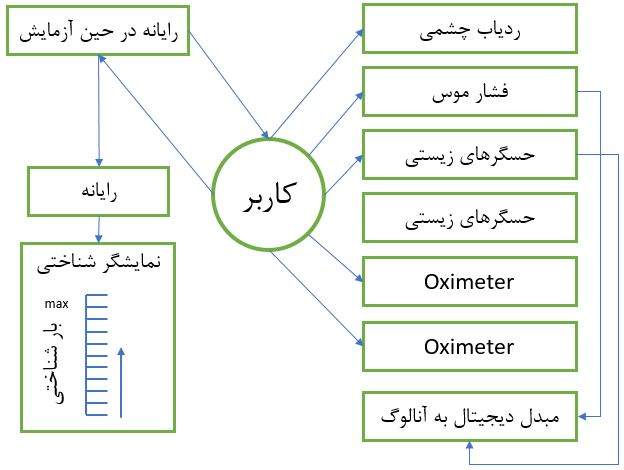
\includegraphics[width=0.7\linewidth]{figures/ikehara2005}
	\caption[نمونه‌ای از سیستم حسگرهای فیزیولوژیکی]{سیستم ها و جریان اطلاعات در آزمایش MTF}
	\label{fig:ikehara2005}
\end{figure}
چِن و همکاران
\cite{Chen2011}
با ۱۲ بسکتبالیست غیرحرفه‌ی ۱۹ تا ۳۶ سال که مبلغی نیز به آن‌ها پرداخت شده بود سعی در اندازه گیری بار شناختی آنها با ۸ داده چشمی داشتند. آزمایش آنها یک برنامه کامپیوتری یادگیری بود، که به کاربر استراتژی بازی را با مشخص کردن مدافعان و مهاجم‌ها و مکانشان نسبت به توپ آموزش می‌داد.
هشت متغیر وابسته برای اندازه‌گیری فشار ذهنی استفاده شدند. شامل: تاخیر در پلک زدن، نرخ پلک زدن، میانگین اندازه مردمک چشم بین ثانیه دوم و انتهای بازی، انحراف معیار در ثانیه چهارم، زمان تثبیت، نرخ تثبیت،‌ اندازه پرش و سرعت پرش چشم.
با توجه به تفاوت در بازه‌ی داده‌های کاربران آنها با رابطه
\eqref{eq:normalize}
در یک بازه قرار می‌دادند.
\begin{equation}\label{eq:normalize}
V_{cal} = \dfrac{V_{raw}-V_{min}}{V_{max}-V_{min}}
\end{equation} 
در پایان مشاهده شد معیارهای مختلف چشمی مثل داده‌هایی که از پلک زدن، حرکت‌های چشم و اندازه مردمک بدست می‌آیند تفاوت روشنی در دو فشار ذهنی کم و زیاد با یک آموزش رایانه‌ای نشان می‌دهد. آنها این معیارها را را قدم اولیه‌ای برای اندازه گیری فشارذهنی به صورت هم زمان معرفی نمودند.
\\

روتستین و همکاران
\cite{ozeri2020relationship}
با برسی ۱۹ کودک بین ۸ تا ۱۲ ساله با زبان مادری انگلیسی که مشکل‌های خواندن داشتند در آزمایشی همراه والدین‌شان به بیمارستان آمده و به آن‌ها دو دسته متن نمایش داده شد، دسته اول جمله‌هایی که پیام و مفهوم خاصی دنبال می‌کنند و دسته دوم جمله‌هایی بدون مفهوم و معنی. به آنها گفته می‌شد تا جایی که امکان دارد درست و سریع پاسخ دهند. با بررسی قطر مردمک چشم و تثبیت توانستند رابطه‌ای میان بارشناختی و داده های چشمی پیدا کنند.

% 6- Concolusion
\section{نتیجه گیری}
\label{s:conclusion}
با بررسی ها و مرور پژوهش‌های انجام شده در این مطالعه می‌توان روی آوردن محققان به سمت داده‌های چشمی را به دلالیل عنوان شده در زیربخش
\ref{ss:ProVsCon}
را مشاهده نمود. از طرفی دستگاه‌ها و سیستم‌های جدید کامپیوتری که انسان در جنبه‌های مختلف زندگی با آن‌ها در ارتباط است به سمت کم حجم شدن و راحتی کاربر می‌روند و یکی از راه‌های ارتباطی چشم انسان است، که می‌تواند داده های بسیار خوبی حتی به صورت هم‌زمان از وضعیت شناختی کاربر بدهد، و این در حالی است که نیازی به دستگاه اضافی و یا مکان خاص نمی‌باشد.
\\
به نظر می‌رسد در صورت انتخاب درست ویژگی‌ها و مشخصه‌های آن  و ترکیب وزن‌دار و یا معمولی آن‌ها می‌توان با دقت خوبی حتی به صورت همزمان وضعیت شناختی کاربر را گزارش نمود.
در شکل
\ref{fig:eyetree}
می‌توانید نمودار درختی انواع داده های چشمی و مشخصه هر کدام را ببینید که تعدادی از آنها به طور کامل در زیربخش
\ref{ss:EyeMeasure}
بررسی شد را ببینید.

\begin{figure}[htbp]
	\centering
	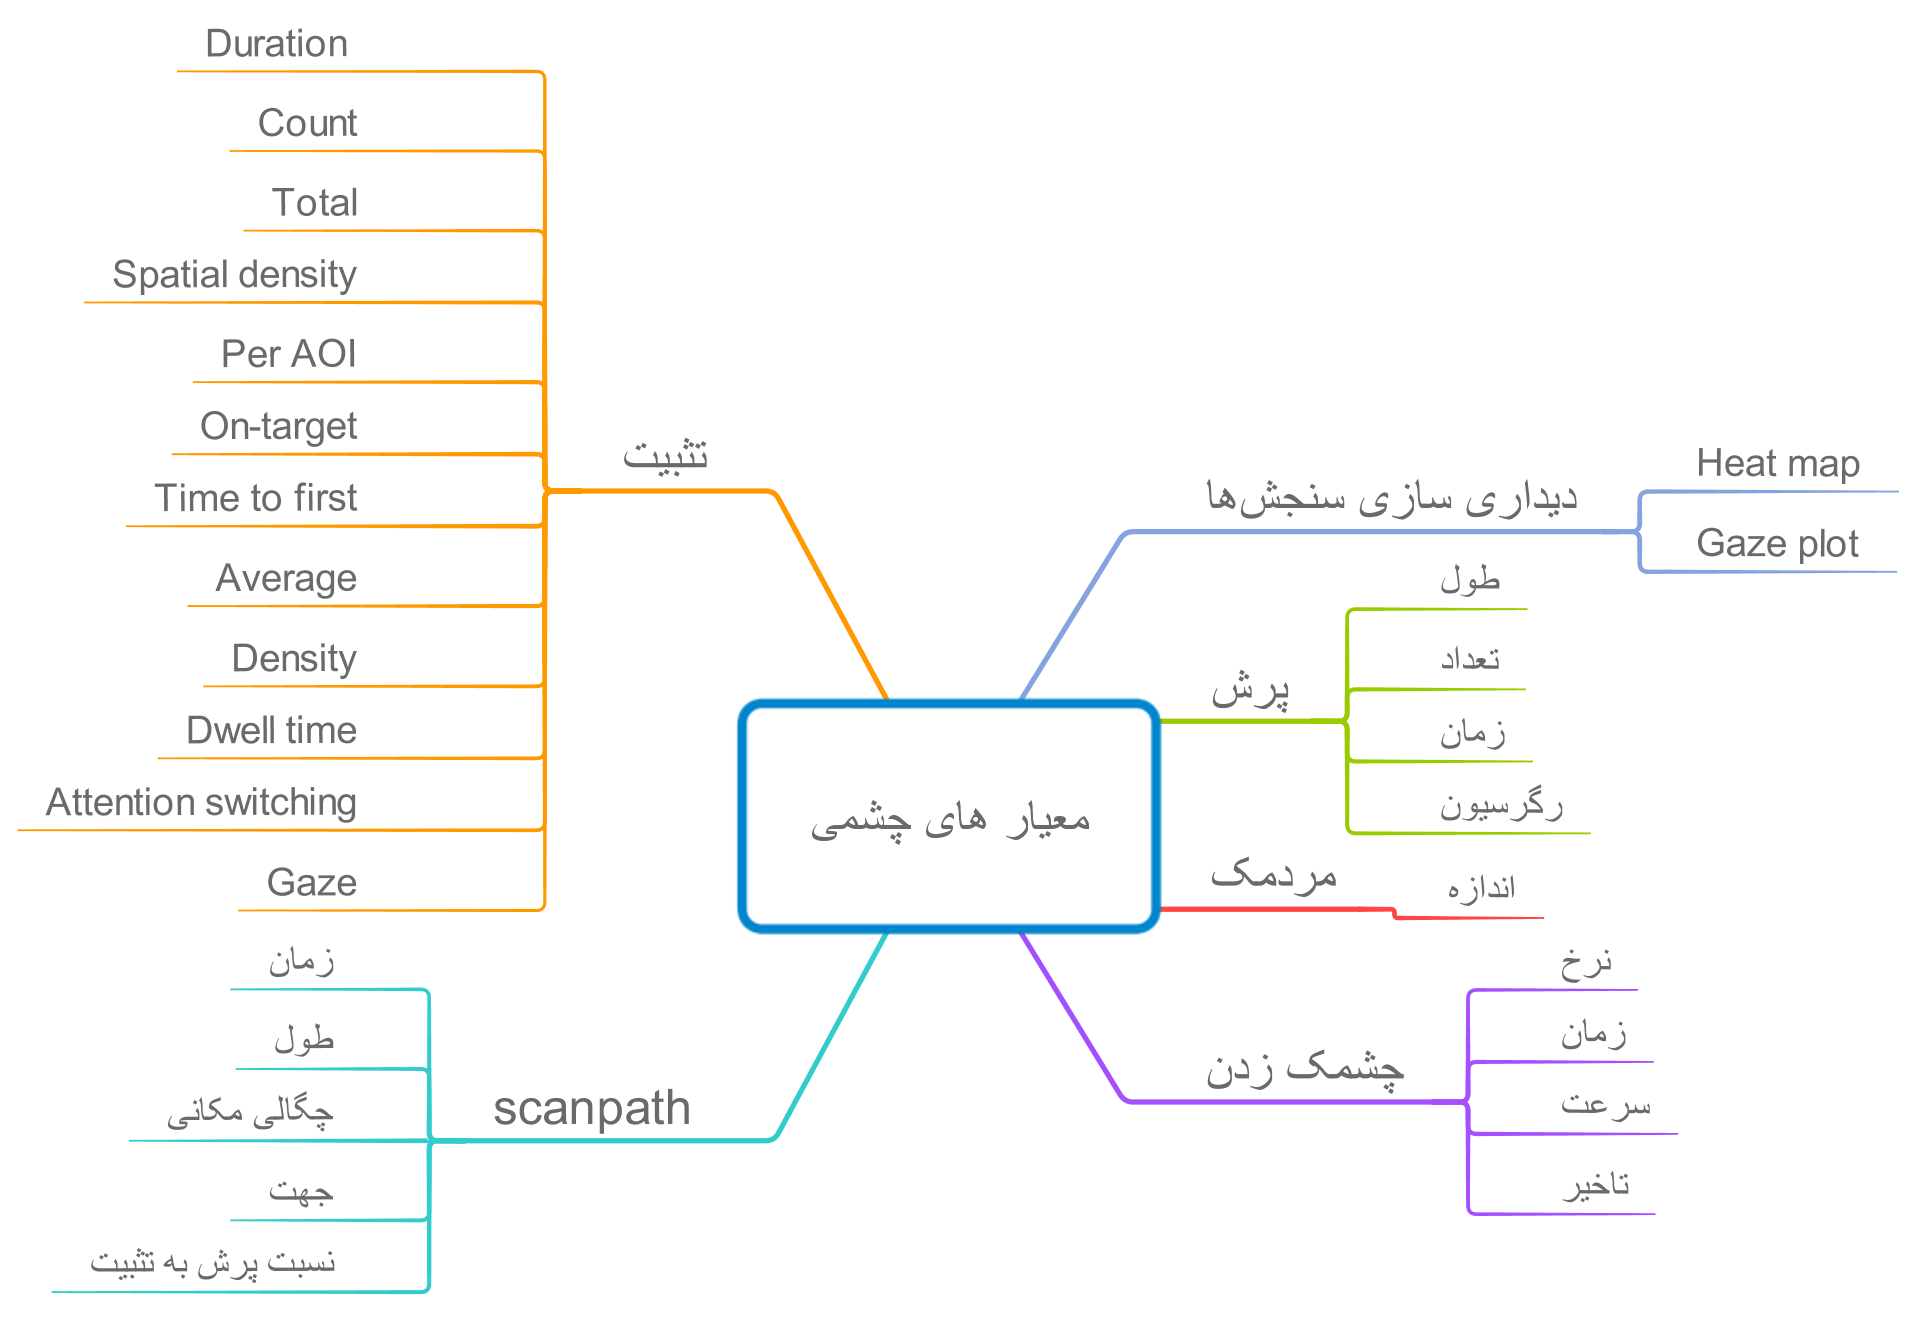
\includegraphics[width=\linewidth]{figures/eye_tree}
	\caption[نمودار درختی داده‌های چشمی]{نمودار درختی انواع داده‌های چشمی و مشخصه هرکدام}
	\label{fig:eyetree}
\end{figure}
جاکوب و همکاران
\cite{Hyona2003}
در پژوهش مروری که انجام دادند میزان استفاده از هریک از داده‌های چشمی در سنجش بار شناختی را گزارش کردند.
در شکل 
\ref{fig:eyedataused}
حاصل گزارش آن‌ها را مشاهده می‌کنید.
\begin{figure}[htbp]
	\centering
	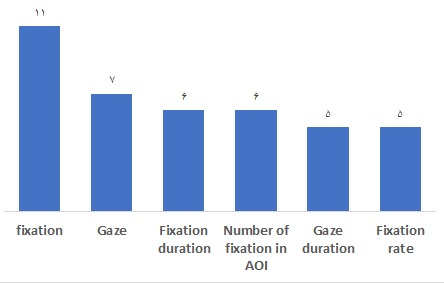
\includegraphics[width=0.7\linewidth]{figures/eyedata_used}
	\caption[میزان استفاده از داده‌های چشمی]{نمودار میزان استفاده از هر یک از داده‌های چشمی}
	\label{fig:eyedataused}
\end{figure}
	

\printindex

%make it left to right
\setLTRbibitems
\bibliographystyle{ieeetr-fa}
\bibliography{references_BIBTEX}

\end{document}